\chapter{Uniform and splayed pretilt profiles}
\label{cha:splay_uniform}
\section{Introduction}
As was shown in chapter \ref{cha:45}, director reorientation under pressure driven flow has been observed via optical conoscopy for the liquid crystal 5CB. In that case, the director was originally oriented at 45$^{\circ}$ to the flow direction and promoted to have planar homogeneous alignment through the rubbed polyimide layer AL-1254 (JSR Corporation). Other initial alignment geometries of the director were also considered, whereby the azimuthal alignment angle (rubbing direction) was set to be at 0$^{\circ}$ (parallel) to the flow direction and at $\approx$ 90$^{\circ}$ (close to normal) to the flow direction.

In this chapter, the effect of the small degree of surface pretilt from the rubbed polyimide layer will be examined in terms of how it affects the average response of the director to flow. Again, optical conoscopy allows us to gain a broad and relatively quick understanding of the average distortions that are taking place. For these experiments, two situations will be considered; \textit{uniform} and \textit{splayed} alignment of the director, which arise from the relative rubbing directions on the bounding surface of the cell. In this study, these effects are examined at a high azimuthal angle of $\phi_0=87^{\circ}$.

\section{Uniform and splayed director profiles}
As will be explained in much greater detail in Chapter \ref{cha:pretilt} (which deals with the physical mechanisms and recipes for producing surface pretilt of the director), when the surface of a planar aligning polyimide is rubbed to promote a planar homogeneous alignment, the shearing force of the rubbing cloth on the surface can permanently deform the aligning layer, leaving a small inclination of the polymer molecules at the surface. As is explained by Geary \textit{et al.} \cite{Geary1987}, if the surface of a polymer is rubbed from left to right, the molecules of the liquid crystal will then tend to align themselves with a slight tilt away from the surface at their right hand ends. This effect is pictorially demonstrated in Figure \ref{fig:uniform_splayed}, whereby the tendency for the liquid crystal molecules to exhibit a small degree of tilt, dependent on the rubbing direction, can be used to create two individual static alignment states, uniform (Figure \ref{fig:uniform_splayed} (a)) and splayed (Figure \ref{fig:uniform_splayed} (b)). The uniform state is created by aligning the surfaces of the cell so that the rubbing directions are anti-parallel to one another and the splayed state is created by aligning the surfaces so that the rubbing directions are parallel to one another\footnote{In Chapter \ref{cha:pretilt}, it will be seen how aligning a cell in the uniform state can be used in a novel technique for measuring the value of the slab tilt angle.}.

\begin{figure}
\begin{center}
\subfigure[Uniform]{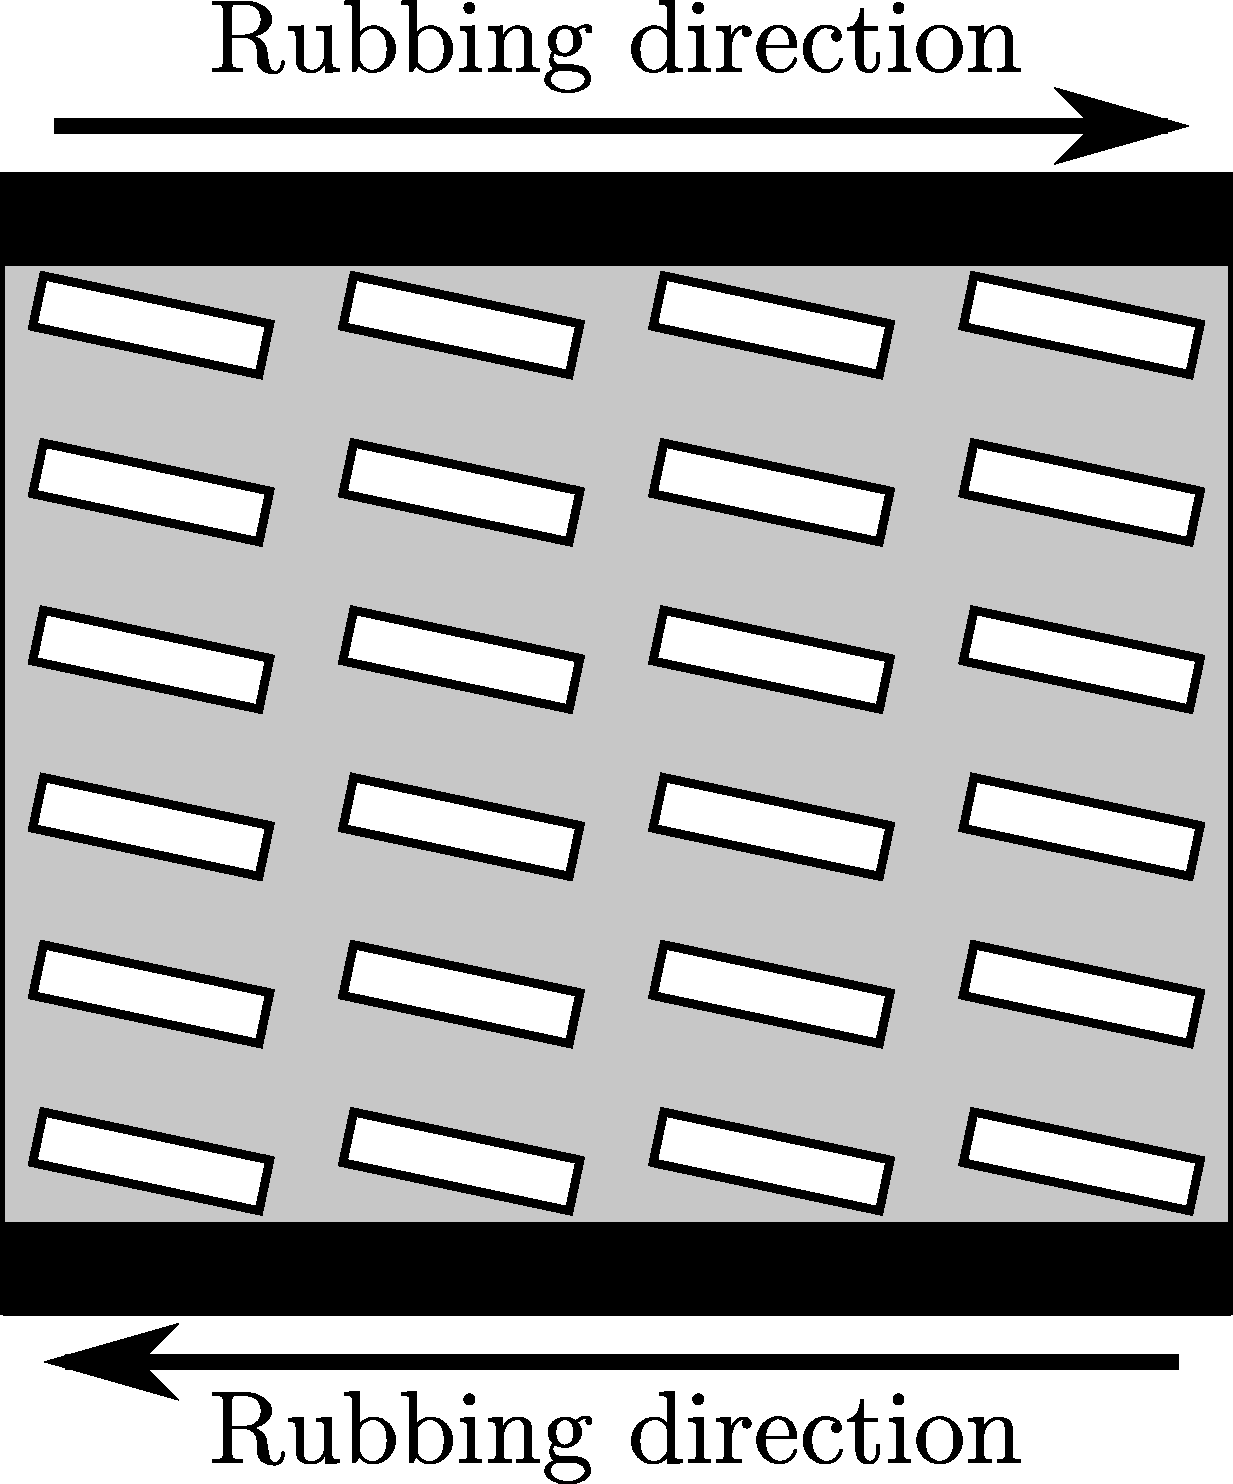
\includegraphics[width=0.3\textwidth]{Figures/90/uniform}}\hspace{0.5in}
\subfigure[Splayed]{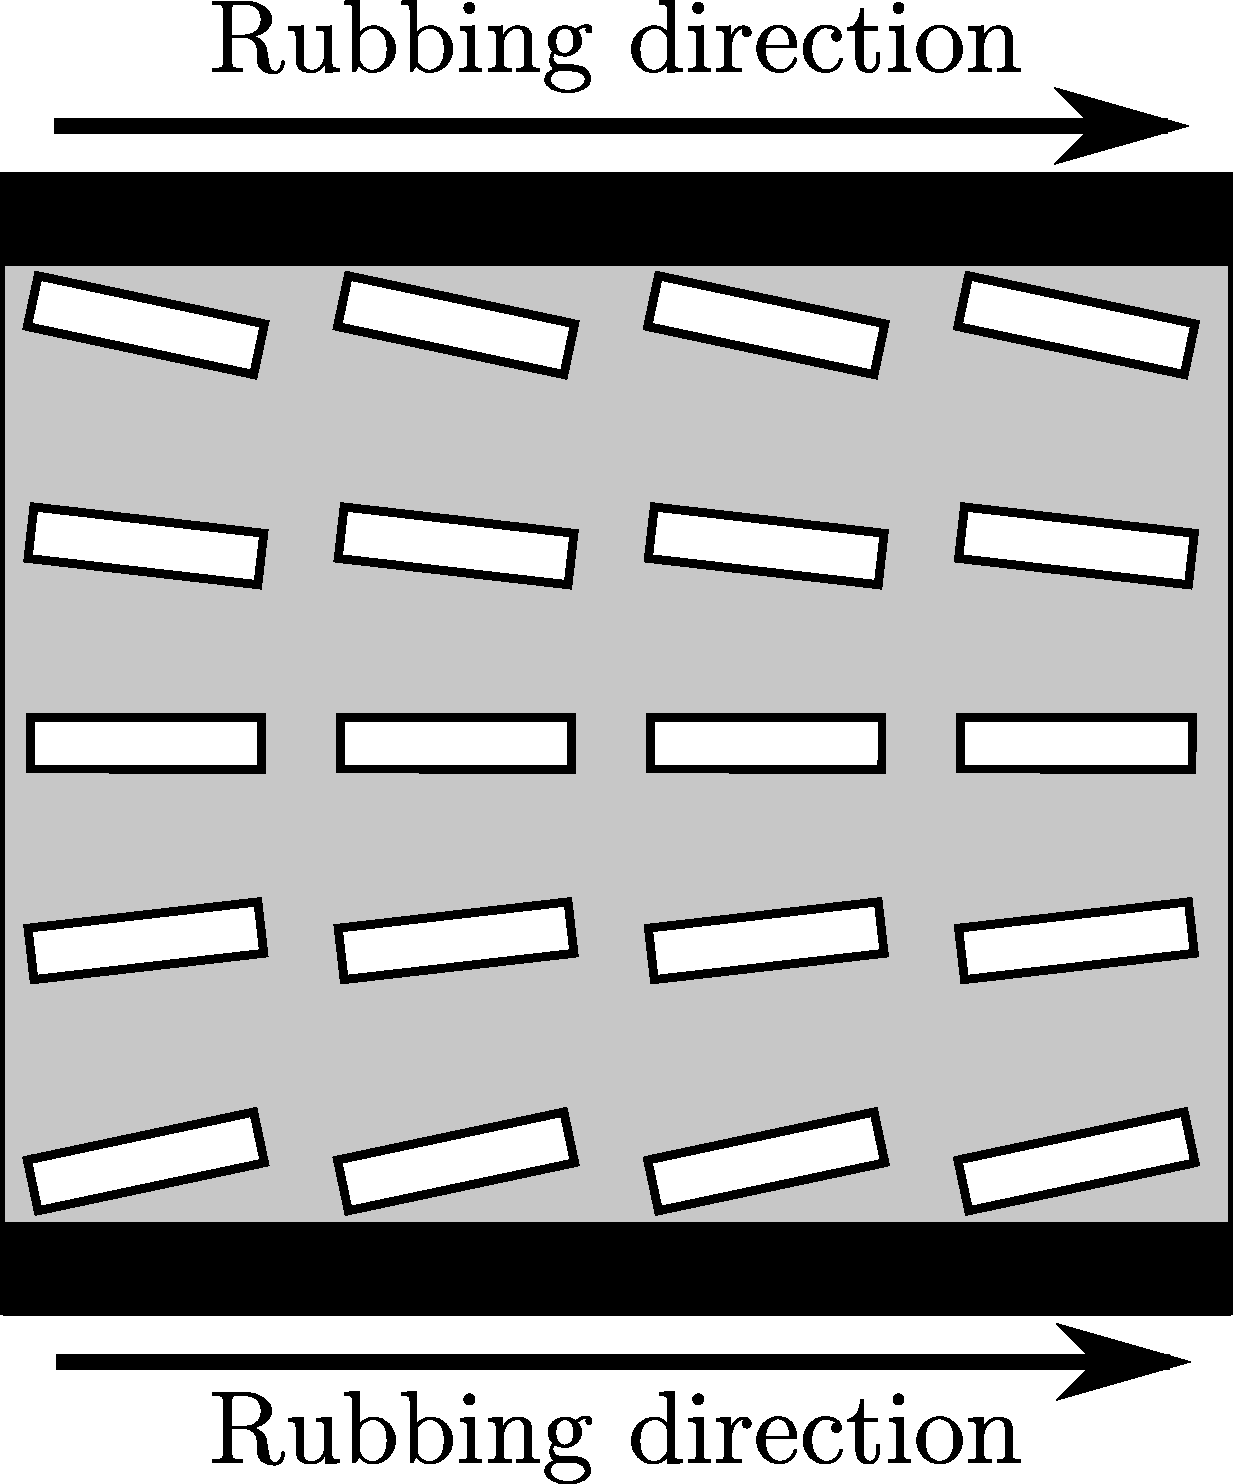
\includegraphics[width=0.3\textwidth]{Figures/90/splay}}
\end{center}
\caption[Schematic diagram of the splayed and uniform states]{\label{fig:uniform_splayed} A schematic diagram depicting the uniform (a) and splayed (b) alignments of the director created by varying the rubbing direction at the cell boundaries (the rubbing direction is indicated by the black arrow). When both surfaces are rubbed parallel, the splayed state is created. When both surfaces are rubbed anti-parallel, the uniform state is created.}
\end{figure}

\section{Uniform tilt alignment}
Generally, the small degree of pretilt that is generated from the rubbing of a planar aligning polyimide layer is on the order of $2^{\circ}$ to $4^{\circ}$ tilted away from the surface. As such (and as is described in Chapter \ref{cha:45}) simulation of the average azimuthal distortion under flow will provide a good and quick estimate to the response of the conoscopic figure. Here, such simulations will be explored to highlight any interesting effects that arise from the uniform pre-tilted alignment state under pressure driven flow.

\subsection{Azimuthal rotation (uniform tilt alignment)}
Figure \ref{fig:90_vary_phi} (a) shows simulated average azimuthal rotation as a function of the volumetric flow rate and initial azimuthal alignment for a cell exhibiting uniform tilt alignment with a value of $\theta=3^{\circ}$ away from the surface. As is expected, for the case of $\phi_0=0^{\circ}$, the director is already aligned parallel to the flow direction (in steady state), and as such, there is no azimuthal rotation of the director observed (black line). As was seen with the curves shown in Chapter \ref{cha:45}, Figure \ref{fig:different_phis}, as the initial azimuthal alignment angle is increased, a rotation of the mean azimuthal distortion is observed as the flow rate is increased, whereby all curves are seen to tend towards the steady state alignment angle of $\phi=0^{\circ}$. As the initial azimuthal angle is increased to a value of $\phi_0=88^{\circ}$ a strikingly different response is seen, whereby rather than distorting towards the steady state angle of $\phi=0^{\circ}$, the average azimuthal alignment goes through a small minimum before rising again towards $\phi=90^{\circ}$. 

This is best shown in Figure \ref{fig:90_vary_phi} (b) which shows a zoom in of Figure \ref{fig:90_vary_phi} (a) with extra curves at varying initial azimuthal alignment angles. Here it is seen that for azimuthal angles above $\phi_0=81^{\circ}$, the average response of the director is to go through a small minimum before increasing towards $\phi=90^{\circ}$. It is important to remember here that Figure \ref{fig:90_vary_phi} is plotting the \textit{average} azimuthal distortion as a function of the flow rate.

\begin{figure}
\begin{center}
\subfigure[]{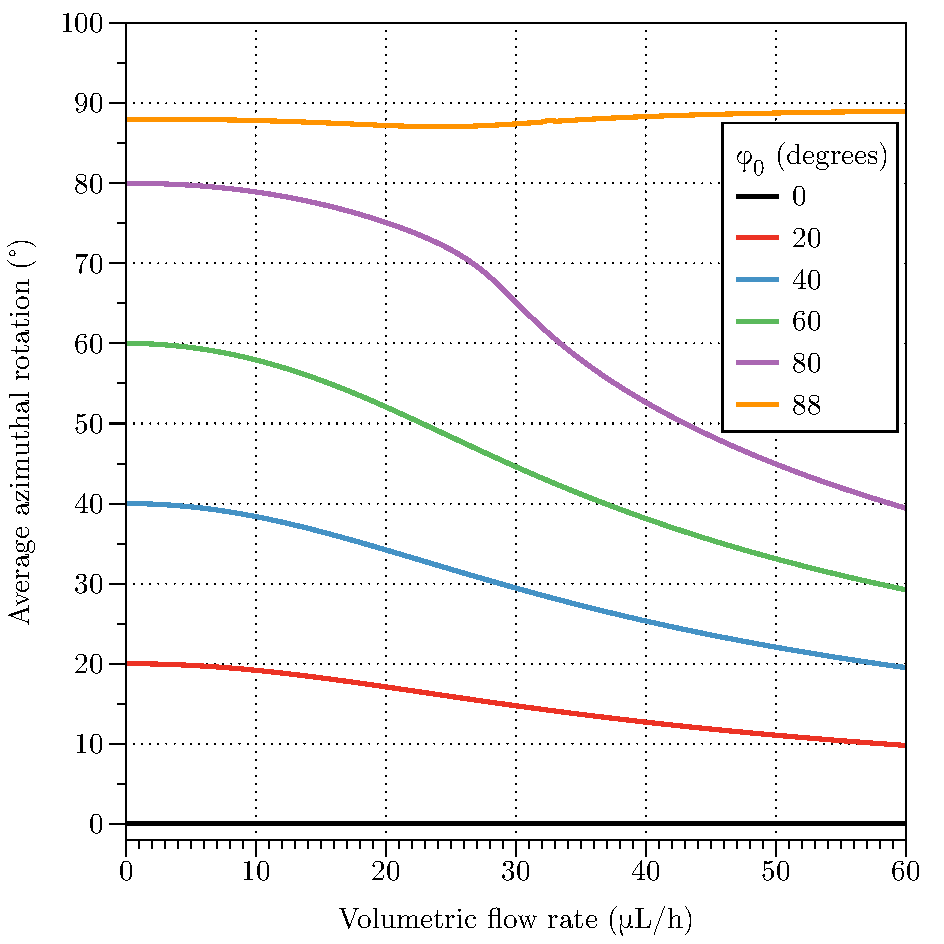
\includegraphics[width=0.49\textwidth]{Figures/90/vary_phi}}
\subfigure[]{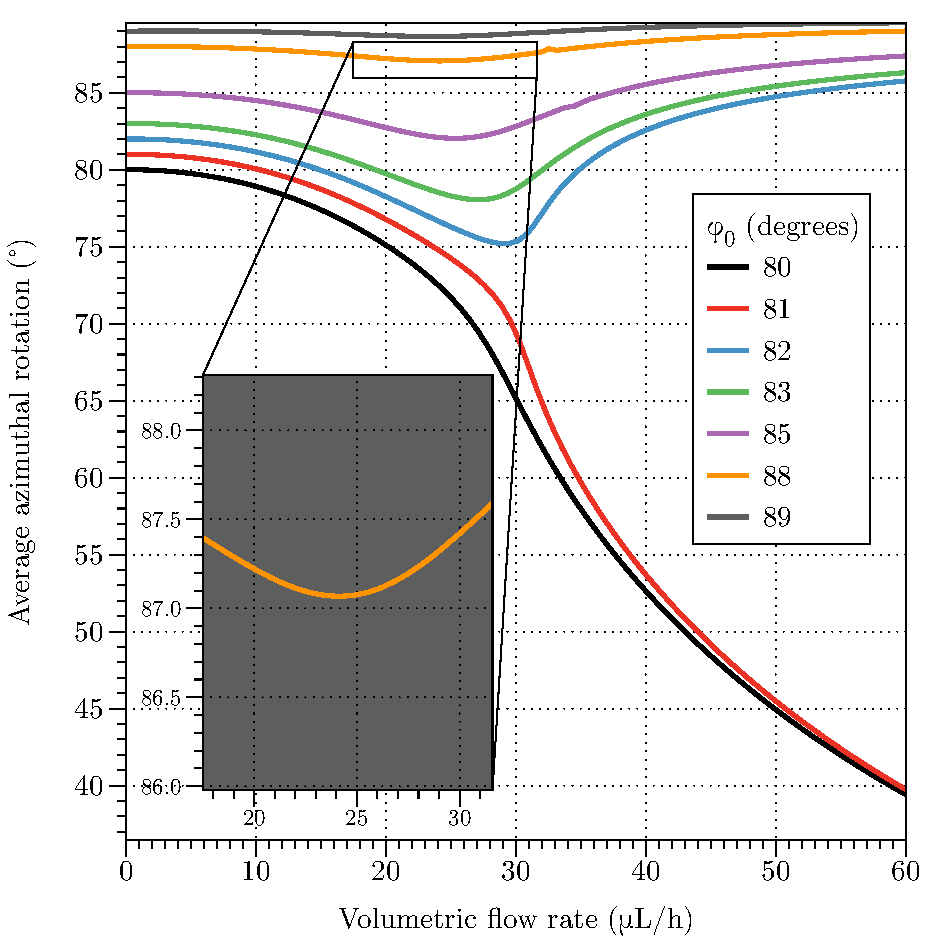
\includegraphics[width=0.49\textwidth]{Figures/90/vary_phi_zoom}}
\end{center}
\caption[Simulated average director rotation for the uniform state]{\label{fig:90_vary_phi} (a) A plot of the simulated azimuthal distortion of the director as a function of the volumetric flow rate and initial azimuthal alignment $\phi_0$. All curves are simulated for the \textit{uniform} tilt alignment with a value of $\theta=3^{\circ}$. As $\phi_0$ increases to values approaching normal to the flow direction, the average azimuthal distortion flattens out. (b) Shows a magnified area of (a) with extra simulated curves. It is seen that as the azimuthal alignment increases above (in this case) $\phi_0=87^{\circ}$, there is a turning point in the curve whereby the average azimuthal distortion increases back towards $90^{\circ}$. The inset in figure (b) shows more clearly the turning point for the $\phi_0=88^{\circ}$ curve.}
\end{figure}

In order to understand the nature and reason behind the minimum that is observed in the average azimuthal rotation, Figure \ref{fig:90_twist_profile_sparce} shows the simulated azimuthal director profile as a function of position in $z$ and pressure gradient (again ranging from no flow (blue) to maximum flow (yellow)) for a cell initially aligned at $\phi_0=87^{\circ}$ exhibiting the uniform tilt profile at an angle of 3$^{\circ}$ away from the surface as simulated in Figure \ref{fig:90_vary_phi}.

\begin{figure}
\begin{center}
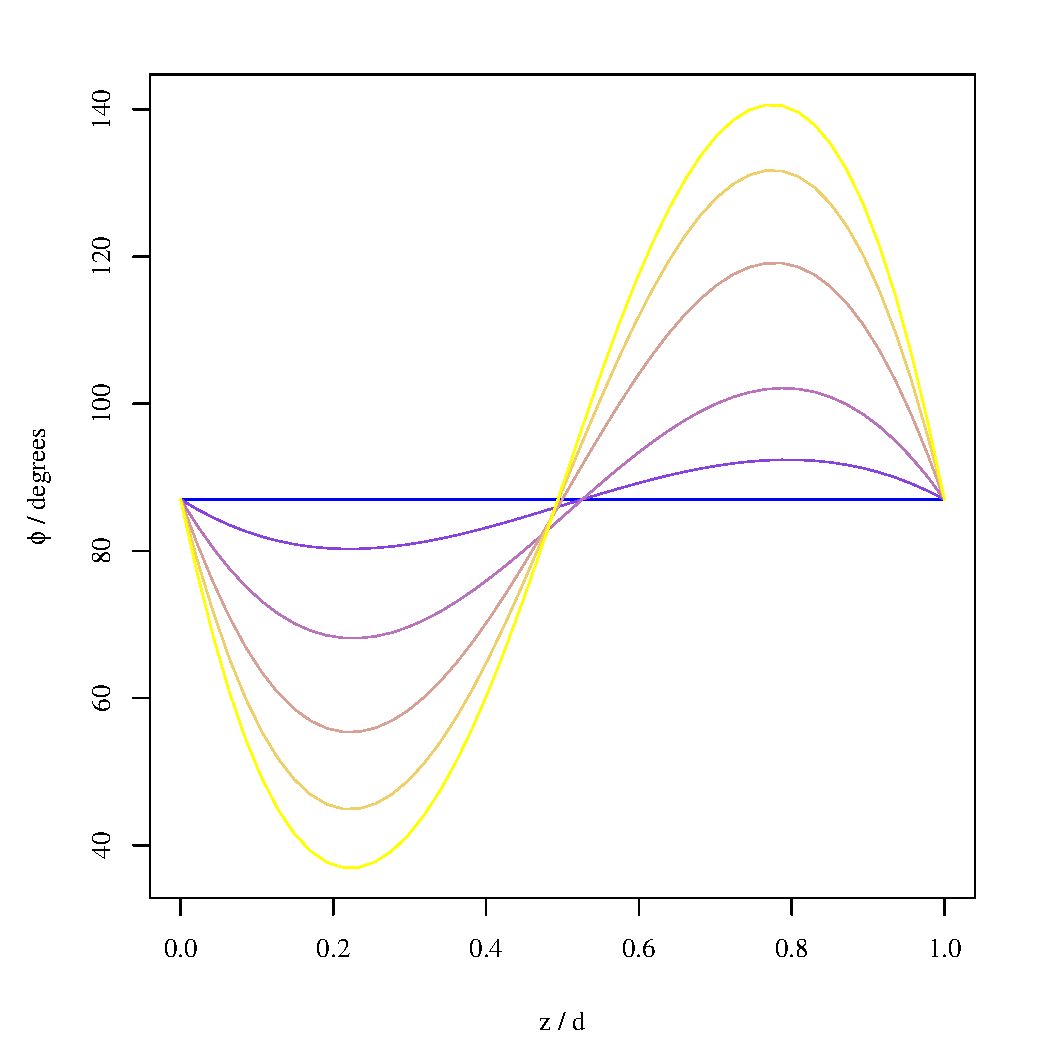
\includegraphics[width=0.7\textwidth]{Figures/90/uniform_twist_profile_sparce}
\end{center}
\caption[Simulated director twist profiles for the uniform state]{\label{fig:90_twist_profile_sparce}Simulated azimuthal director profile for a cell aligned at $\phi_0=87^{\circ}$. As shown before, blue indicates no flow, moving through to yellow at maximum flow. It is clear that the director distorts in opposite directions about the cell mid-plane. The magnitude of this distortion away from $\phi_0=87^{\circ}$ is seen to be asymmetric at lower flow rates before becoming symmetric about $z=d/2$ at higher flow rates.}
\end{figure}

This figure demonstrates that the director is simulated to rotate in opposite directions about the cell mid-plane under flow. Crucially, at lower flow rates, this reversal in rotation direction does not occur at exactly the cell mid-plane. This is demonstrated in Figure \ref{fig:90_twist_profile_sparce} whereby at lower flow rates, more than half of the cell is rotating towards $\phi=0^{\circ}$. This asymmetry in the magnitude of the azimuthal distortion results in the \textit{average} value (plotted in Figure \ref{fig:90_vary_phi}) to dip towards the value of $\phi=0^{\circ}$. As the flow rate is increased, this asymmetry in the direction of director rotation reduces, with both halves of the cell now rotating in opposite directions about the cell mid-plane (yellow line). The symmetry of the distortion about $z=d/2$ at higher flow rates results in the average azimuthal distortion increasing to come back towards $\phi=90^{\circ}$. It is for this reason that the small turning point observed in Figure \ref{fig:90_vary_phi} exists.

In other words, the director can be thought of as azimuthally distorting in one direction (here termed the negative direction, as $\phi$ is decreasing towards $0^{\circ}$) in more than one half of the cell, while the remainder of the cell distorts azimuthally in the opposite direction (here termed the positive direction, as $\phi$ is increasing towards $180^{\circ}$) but by a lesser amount. This difference creates the small overall azimuthal distortion in the negative direction. At increased flow rates this effect is reversed, with more than half of the cell azimuthally distorting in the positive direction and the remainder of the cell distorting in the negative direction, with the overall effect being an increase in the average azimuthal distortion and the creation of the turning point seen in Figure \ref{fig:90_vary_phi}. 

An analysis and full discussion of this phenomenon and its effect will be given later in the analysis of the simulated director profiles (Section \ref{sec:uniform_state_analysis}).

\section{Experiment}
\label{sec:uniform_experiment}
In order to experimentally probe the response shown above for the pressure driven flow of 5CB in the uniformly tilted state, simulation of the optimal alignment conditions were made in order to maximise the chance of observing the small azimuthal minimum in the conoscopic figure's rotation. As such, it was estimated that the rubbed polymer alignment layer may give $2^{\circ}$ pretilt away from the surface as a result of rubbing. In this case, the strength of contact between the slide and the rubbing cloth was also slightly increased in order to promote a slightly larger pretilt angle than might normally be achieved. Figure \ref{fig:vary_tilt}(a) shows how the simulated response changes as a function of initial azimuthal alignment $\phi_0$ for a cell exhibiting $2^{\circ}$ pretilt in the uniform state. It is clear that the optimal azimuthal alignment angle to use is that of $\phi_0=87^{\circ}$, as this produces the deepest minimum, ranging from $\phi=87^{\circ}$ to $\phi\approx82.5^{\circ}$ (blue line). For higher values of $\phi_0$, the depth of the minimum is considerably less. Figure \ref{fig:vary_tilt}(b) shows the average azimuthal response for an initial azimuthal alignment of $\phi_0=87^{\circ}$ with varying degrees of pretilt, ranging from $2^{\circ}$ to $5^{\circ}$ tilted away from the surface. It is seen that a pretilt angle of $2^{\circ}$ would also provide the deepest minimum in the average response.

\begin{figure}
\begin{center}
\subfigure[]{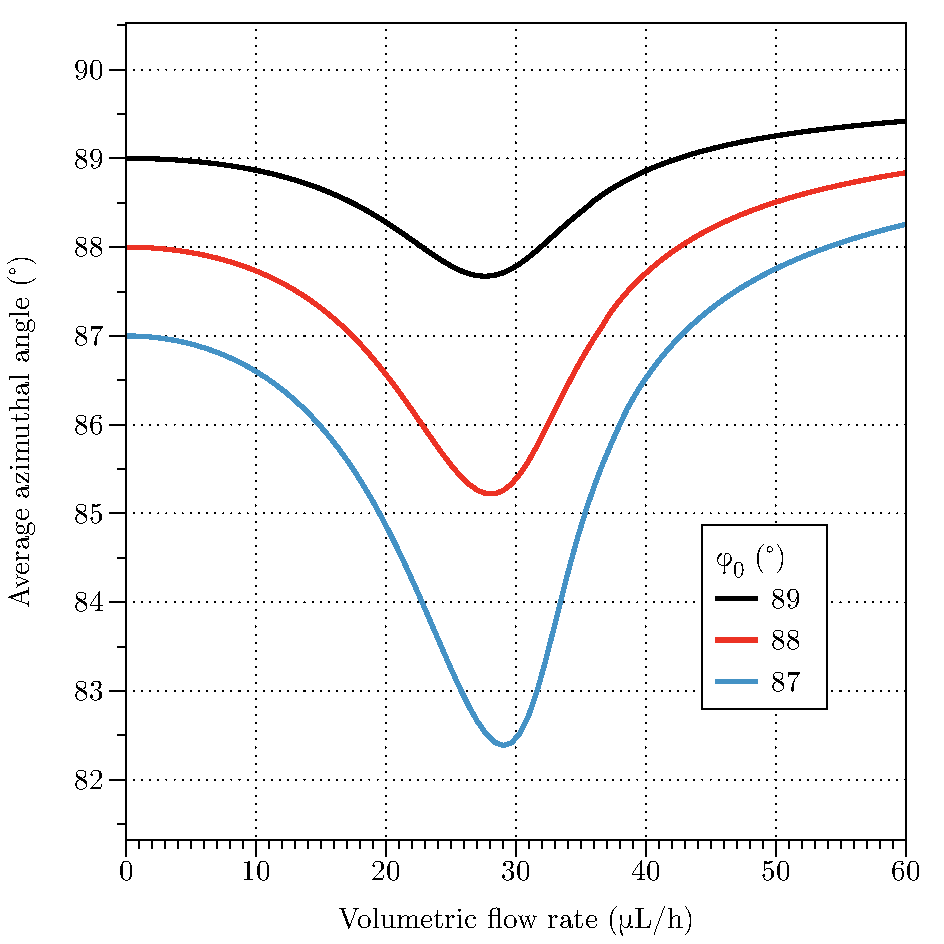
\includegraphics[width=0.49\textwidth]{Figures/90/2tilt_vary_phi}}
\subfigure[]{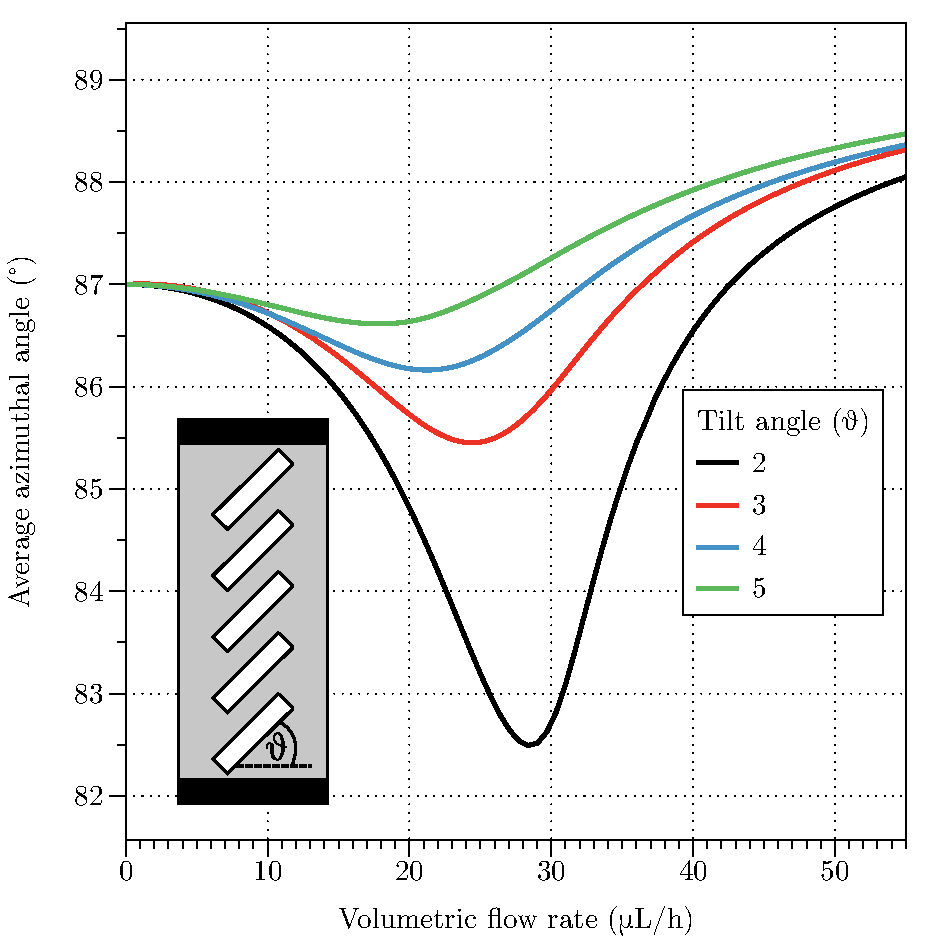
\includegraphics[width=0.49\textwidth]{Figures/90/uniform_vary_tilt}}
\end{center}
\caption[Optimising values of $\phi_0$ and $\theta_0$ for uniform state]{\label{fig:vary_tilt}(a) Shows how the average response varies as a function of the initial azimuthal alignment angle $\phi_0$ for a cell exhibiting $2^{\circ}$ pretilt in the uniform state. The deepest minimum is seen for an azimuthal alignment angle of $\phi_0=87^{\circ}$. (b) Shows how the average response varies as a function of the tilt angle in the uniform state for an initial azimuthal alignment of $\phi_0=87^{\circ}$.}
\end{figure}

Following this analysis, a flow cell was fabricated, as described in Chapter \ref{sec:theory}, Section \ref{sec:cell_construction}, using Optimer AL1254 (JSR corporation) as the alignment layer, rubbed at $\phi_0=87^{\circ}$ and assembled such that the rubbing directions are aligned anti-parallel to one another. Figure \ref{fig:uniform_data} shows the experimental conoscopic figures as a function of the volumetric flow rate set at the syringe drive (given in the caption of each individual figure). Immediately it is evident that the conoscopic figures in this study vary from those shown in Chapter \ref{cha:45}. Considering just the static, non-flowing conoscopic figure (Figure \ref{fig:uniform_data}(a)), it is clear that the centre of the conoscopic figure is translated away from the centre of the field of view. This is evident from the bottom black band of the conoscopic figure only just being visible in the field of view. As will be discussed later, this translation is due to the uniform tilt angle through the depth of the cell as schematically shown in Figure \ref{fig:uniform_splayed}(a). As the flow rate is increased, this translation of the conoscopic figure is further exaggerated with the centre of the conoscopic figure no longer being visible at the largest flow rates. 

As is also shown by the red lines in Figures \ref{fig:uniform_data} (a), (h) and (m), the azimuthal alignment of the conoscopic figure also goes through a small minimum (shown clearly later in Figure \ref{fig:uniform_data_plot}) whereby it rotates a small amount in the clockwise direction as the flow rate is increased to approximately $28\mu L/h$ before rotating back towards the initial azimuthal alignment at approximately $48\mu L/h$. These results will be discussed later in the conclusions of the Chapter.


\begin{figure}
\begin{center}
\subfigure[0 $\mu$L/h]{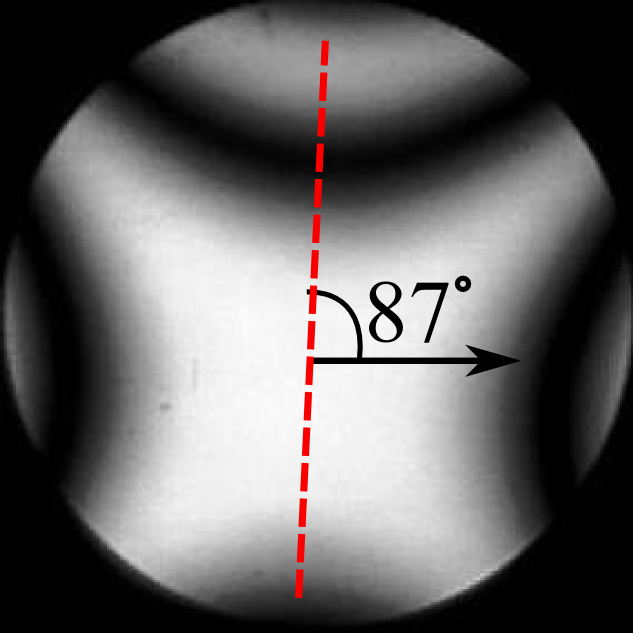
\includegraphics[width=0.17\textwidth]{Figures/90/parallel/data/leveled/00a}}
%\subfigure[2 $\mu$L/h]{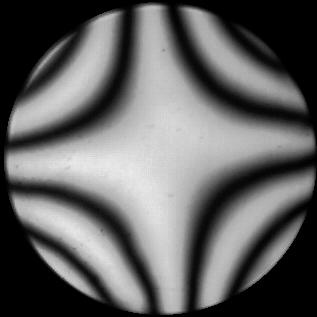
\includegraphics[width=0.17\textwidth]{Figures/90/parallel/data/leveled/01}}
\subfigure[4 $\mu$L/h]{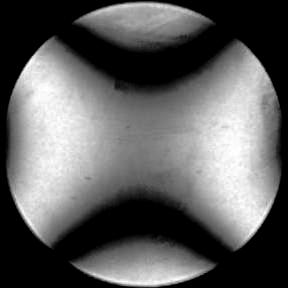
\includegraphics[width=0.17\textwidth]{Figures/90/parallel/data/leveled/02}}
%\subfigure[6 $\mu$L/h]{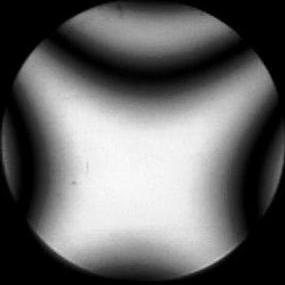
\includegraphics[width=0.17\textwidth]{Figures/90/parallel/data/leveled/03}}
\subfigure[8 $\mu$L/h]{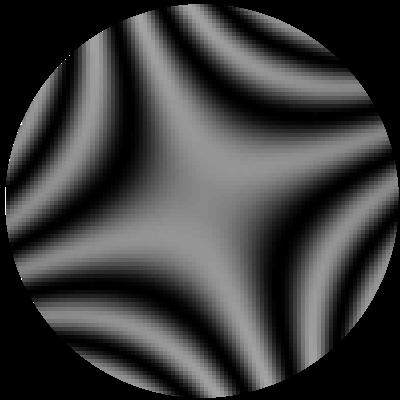
\includegraphics[width=0.17\textwidth]{Figures/90/parallel/data/leveled/04}}
%\subfigure[10 $\mu$L/h]{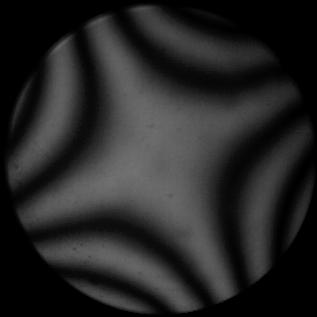
\includegraphics[width=0.17\textwidth]{Figures/90/parallel/data/leveled/05}}
\subfigure[12 $\mu$L/h]{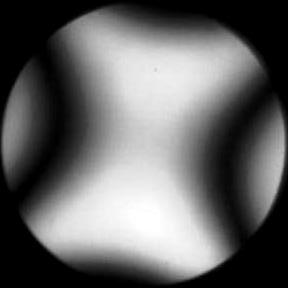
\includegraphics[width=0.17\textwidth]{Figures/90/parallel/data/leveled/06}}
%\subfigure[14 $\mu$L/h]{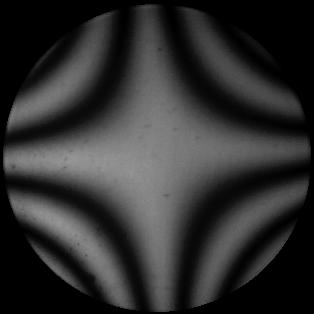
\includegraphics[width=0.17\textwidth]{Figures/90/parallel/data/leveled/07}}
\subfigure[16 $\mu$L/h]{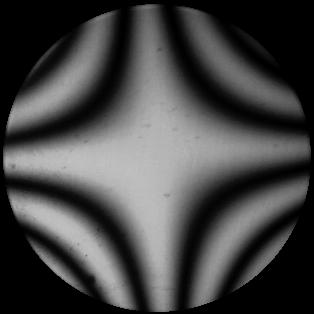
\includegraphics[width=0.17\textwidth]{Figures/90/parallel/data/leveled/08}}
%\subfigure[18 $\mu$L/h]{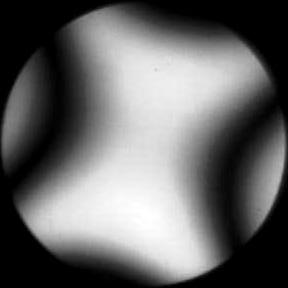
\includegraphics[width=0.17\textwidth]{Figures/90/parallel/data/leveled/09}}
\subfigure[20 $\mu$L/h]{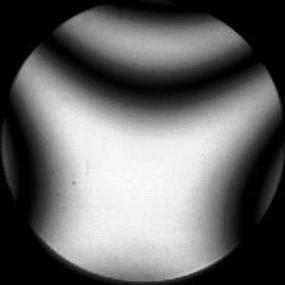
\includegraphics[width=0.17\textwidth]{Figures/90/parallel/data/leveled/10}}
%\subfigure[22 $\mu$L/h]{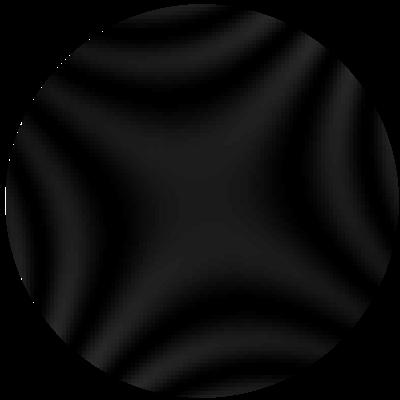
\includegraphics[width=0.17\textwidth]{Figures/90/parallel/data/leveled/11}}
\subfigure[24 $\mu$L/h]{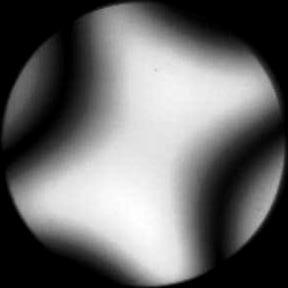
\includegraphics[width=0.17\textwidth]{Figures/90/parallel/data/leveled/12}}
%\subfigure[26 $\mu$L/h]{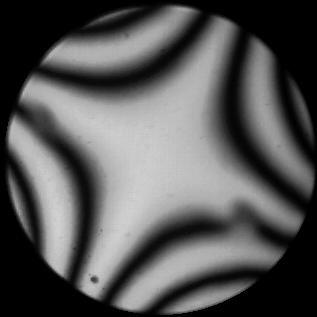
\includegraphics[width=0.17\textwidth]{Figures/90/parallel/data/leveled/13}}
\subfigure[28 $\mu$L/h]{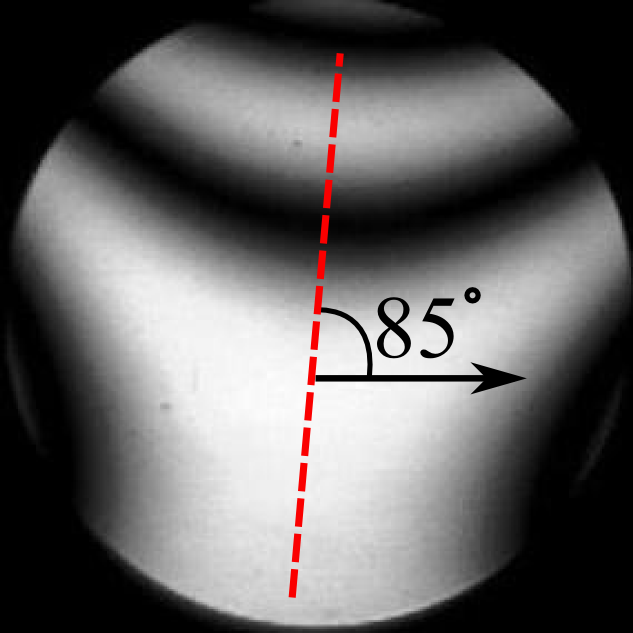
\includegraphics[width=0.17\textwidth]{Figures/90/parallel/data/leveled/14a}}
%\subfigure[30 $\mu$L/h]{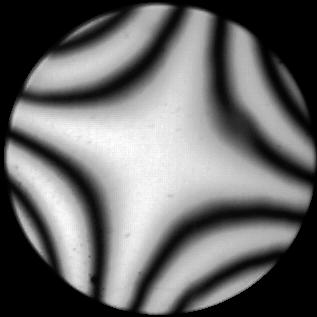
\includegraphics[width=0.17\textwidth]{Figures/90/parallel/data/leveled/15}}
\subfigure[32 $\mu$L/h]{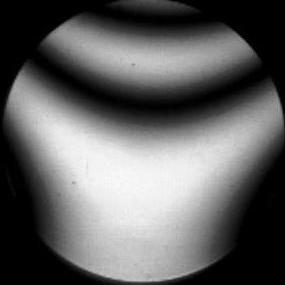
\includegraphics[width=0.17\textwidth]{Figures/90/parallel/data/leveled/16}}
%\subfigure[34 $\mu$L/h]{\includegraphics[width=0.17\textwidth]{Figures/90/parallel/data/leveled/17}}
\subfigure[36 $\mu$L/h]{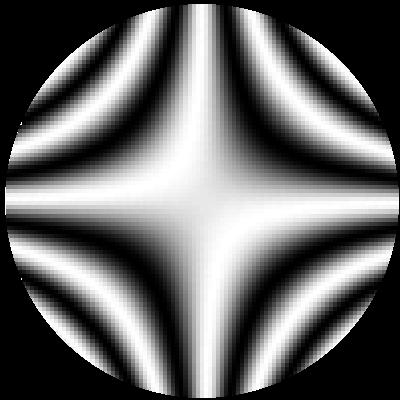
\includegraphics[width=0.17\textwidth]{Figures/90/parallel/data/leveled/18}}
%\subfigure[38 $\mu$L/h]{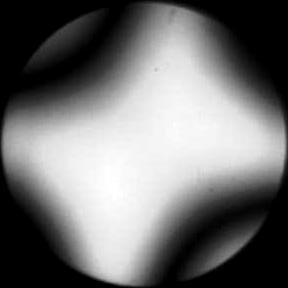
\includegraphics[width=0.17\textwidth]{Figures/90/parallel/data/leveled/19}}
\subfigure[40 $\mu$L/h]{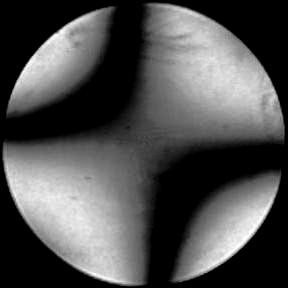
\includegraphics[width=0.17\textwidth]{Figures/90/parallel/data/leveled/20}}
%\subfigure[42 $\mu$L/h]{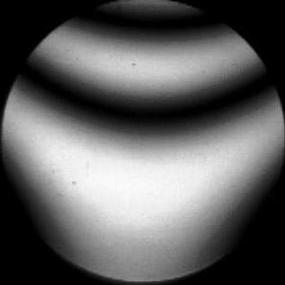
\includegraphics[width=0.17\textwidth]{Figures/90/parallel/data/leveled/21}}
\subfigure[44 $\mu$L/h]{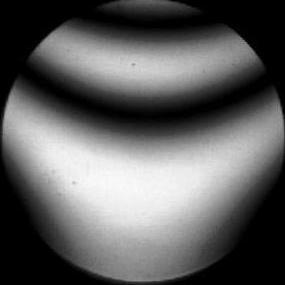
\includegraphics[width=0.17\textwidth]{Figures/90/parallel/data/leveled/22}}
%\subfigure[46 $\mu$L/h]{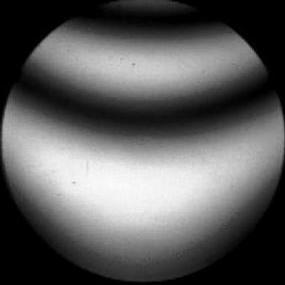
\includegraphics[width=0.17\textwidth]{Figures/90/parallel/data/leveled/23}}
\subfigure[48 $\mu$L/h]{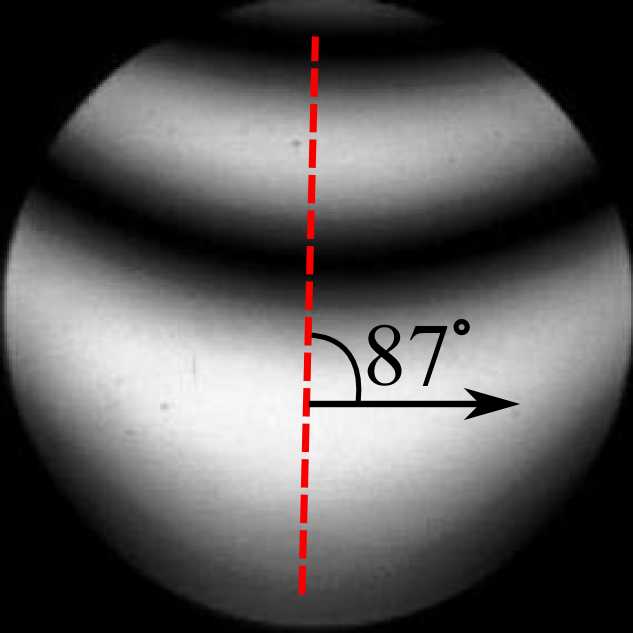
\includegraphics[width=0.17\textwidth]{Figures/90/parallel/data/leveled/24a}}
%\subfigure[50 $\mu$L/h]{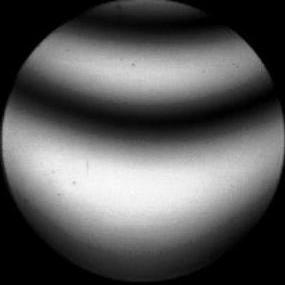
\includegraphics[width=0.17\textwidth]{Figures/90/parallel/data/leveled/25}}
\subfigure[]{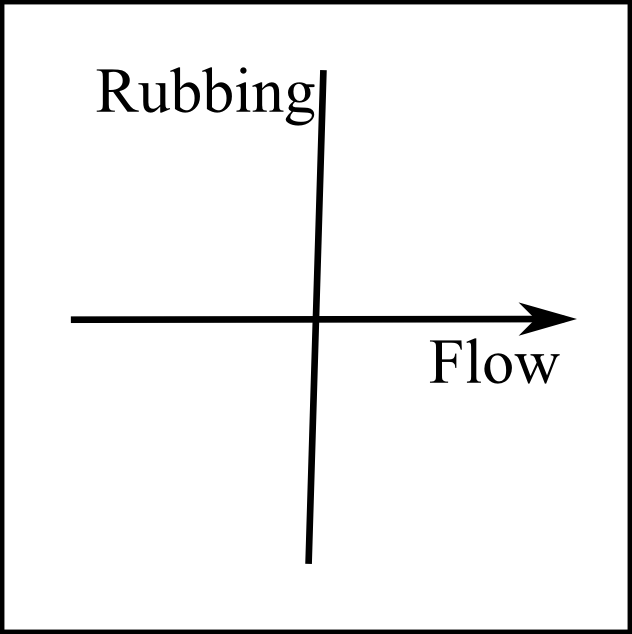
\includegraphics[width=0.17\textwidth]{Figures/90/parallel/data/leveled/coords}}
\end{center}
\caption[Experimental conoscopic figures for the uniformly aligned state]{\label{fig:uniform_data}Experimental conoscopic interference figures for the cell rubbed at $\phi_0=87^{\circ}$ in the anti-parallel (uniformly tilted) geometry. Here, a small rotation minimum of the conoscopic figure as a function of the volumetric flow rate set by the syringe drive (shown in the individual figure caption) is observed.}
%\begin{center}
%%\rule{3in}{0.5pt}
%\end{center}
\end{figure}

\subsection{Estimating the crystal pretilt angle}
\label{sec:calc_tilt}
As is described by Van Horn and Henning Winter in their 2001 publication \cite{Horn2001}, an estimate of the liquid crystal slab tilt angle can be made when the symmetrical centre of the conoscopic figure is visible (as is the case here, as discussed above, for the static, non-flowing conoscopic figure depicted in Figure \ref{fig:uniform_data}(a)). Their novel method (which is a substantial improvement and simplification on previous cumbersome techniques) uses Mallard's equation \cite{Mallard1882,Horn2001} to calculate the angle between the surface normal and the ray of light that forms the origin of the interference figure, $\alpha_0$, as is shown below (equation \ref{eq:mallards}),

\begin{equation}
\label{eq:mallards}
\frac{r}{R}\text{NA}=\langle n\rangle\sin\left(\alpha_0\right)
\end{equation}

\noindent where $r$ is the distance between the centre of the field of view and the centre of the conoscopic figure, $R$ is the radius of the field of view, NA is the numerical aperture of the objective lens and $\langle n\rangle$ is the mathematical average of the refractive index through the sample. Once the angle $\alpha_0$ has been calculated, the slab tilt angle $\theta$ (measured from the surface) can be determined from the appropriate phase difference equation for uniaxial crystals \cite{Horn2001}. For the case of a near planar aligned sample exhibiting only a small pretilt angle, this equation takes the form\footnote{For an in depth and full analysis of this method for estimating uniaxial tilt angles from the conoscopic figure, the reader is directed to the publication by Van Horn and Henning Winter titled \textit{Analysis of the conoscopic measurement for uniaxial liquid-crystal tilt angles} \cite{Horn2001}},

\begin{equation}
\label{eq:vanhorn}
\theta=\tan^{-1}\left(\frac{-\sin\left(2\alpha_0\right)}{3+\cos\left(2\alpha_0\right)}\right)
\end{equation}

\begin{figure}
\begin{center}
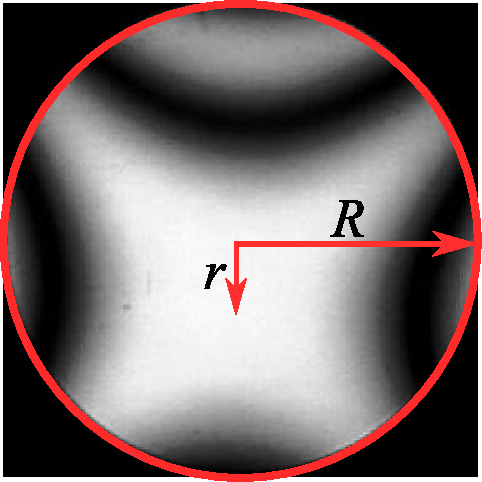
\includegraphics[width=0.3\textwidth]{Figures/90/calculate_tilt_pdf}
\end{center}
\caption[Estimation of the uniform tilt angle from the conoscopic figure]{\label{fig:calculate_tilt}The 0 $\mu L/h$ experimental conoscopic figure (image (a) in Figure \ref{fig:uniform_data}). The radius of the field of view $R$ and the distance from the centre of the circle to the centre of the conoscopic figure $r$ are shown. The ratio of these two lengths can be used to estimate the tilt angle of the cell from equations \ref{eq:mallards} and \ref{eq:vanhorn}. For this figure, the ratio $r/R=0.29$, $\text{NA}=0.55$ and $\langle n\rangle\approx1.6$, resulting in a slab tilt angle of $\theta\approx3^{\circ}$ away from the surface.}
\end{figure}

\noindent Figure \ref{fig:calculate_tilt} shows the static, non-flowing, conoscopic figure for the cell aligned at $\phi_0=87^{\circ}$ with the uniform slab tilt angle produced from the anti-parallel rubbing directions. The perimeter of the field of view, and the distances $r$ and $R$ are shown. In this case, $r/R=0.29$, $\text{NA}=0.55$ and $\langle n\rangle\approx1.6$. Following from equations \ref{eq:mallards} and \ref{eq:vanhorn}, a value of $\alpha_0=5.8^{\circ}$ and $\theta\approx3^{\circ}$ is obtained. Therefore, a rough estimate of the \textit{average} pretilt angle exhibited in the cell has been made, resulting in a value of $\theta\approx3^{\circ}$ tilted away from the aligning surfaces. As is also mentioned in the analysis by Van Horn and Henning Winter, this technique can only be used to a first approximation for small tilt angles of uniform director tilt profiles, whereby a primary source of error is the measurement of $r$ (which could yield results to within a fraction of a degree depending on the technique and optical setup) \cite{Horn2001}. In this case, it is suitable and provides a reliable estimate for the uniform tilt angle present in the cell.

\subsection{Conoscopic figure rotation}
\label{sec:uniform_con_rot}
Figure \ref{fig:uniform_rotation} shows plots from the automated routine for measuring the azimuthal angle of the conoscopic figure. Here, the azimuthal angle of the 20 $\mu L/h$ figure is found (Figure \ref{fig:uniform_data} (f)). Again, it is clear that the difference between the pixel intensities for the two test lines has been minimised at an angle of $\phi\approx84^{\circ}$ from the figure's $x$ axis.

\begin{figure}
\begin{center}
\subfigure[]{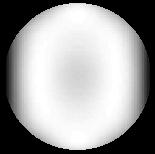
\includegraphics[width=0.38\textwidth]{Figures/90/uniform_rotation/1}}\hspace{0.3in}
\subfigure[]{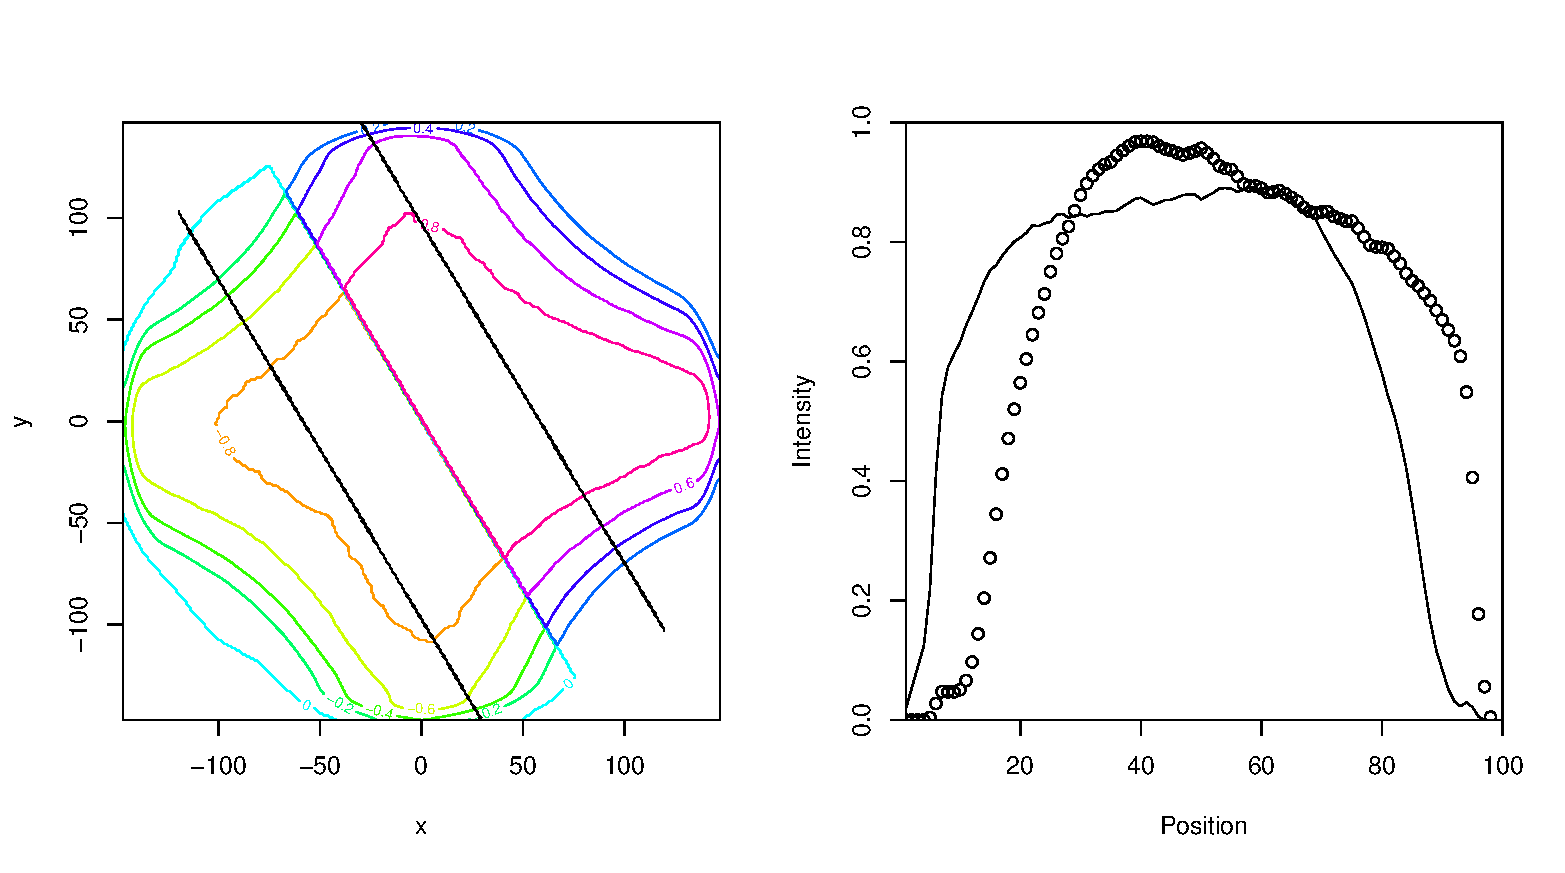
\includegraphics[width=0.38\textwidth]{Figures/90/uniform_rotation/2}}
\subfigure[]{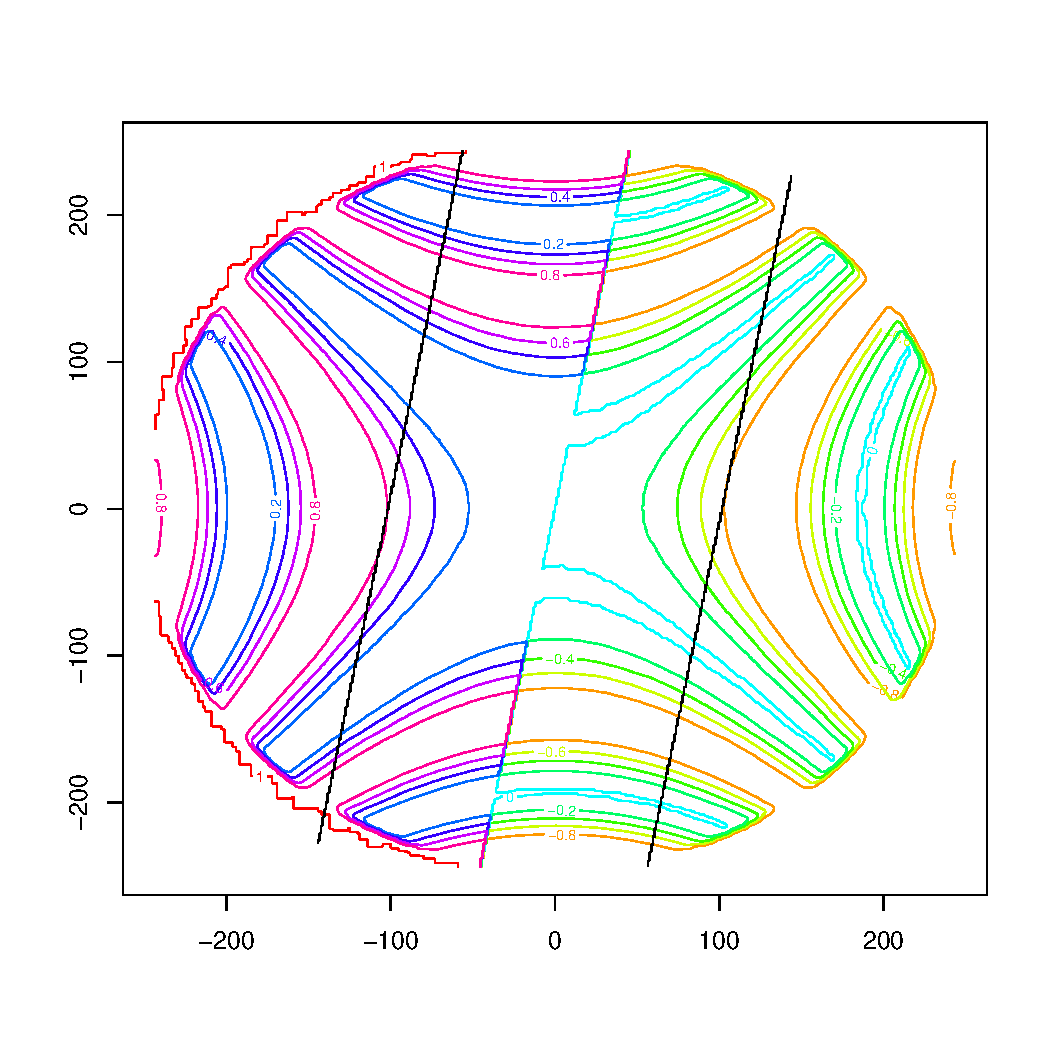
\includegraphics[width=0.38\textwidth]{Figures/90/uniform_rotation/3}}\hspace{0.3in}
\subfigure[]{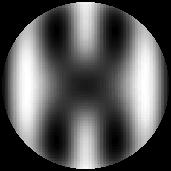
\includegraphics[width=0.38\textwidth]{Figures/90/uniform_rotation/4}}
\subfigure[]{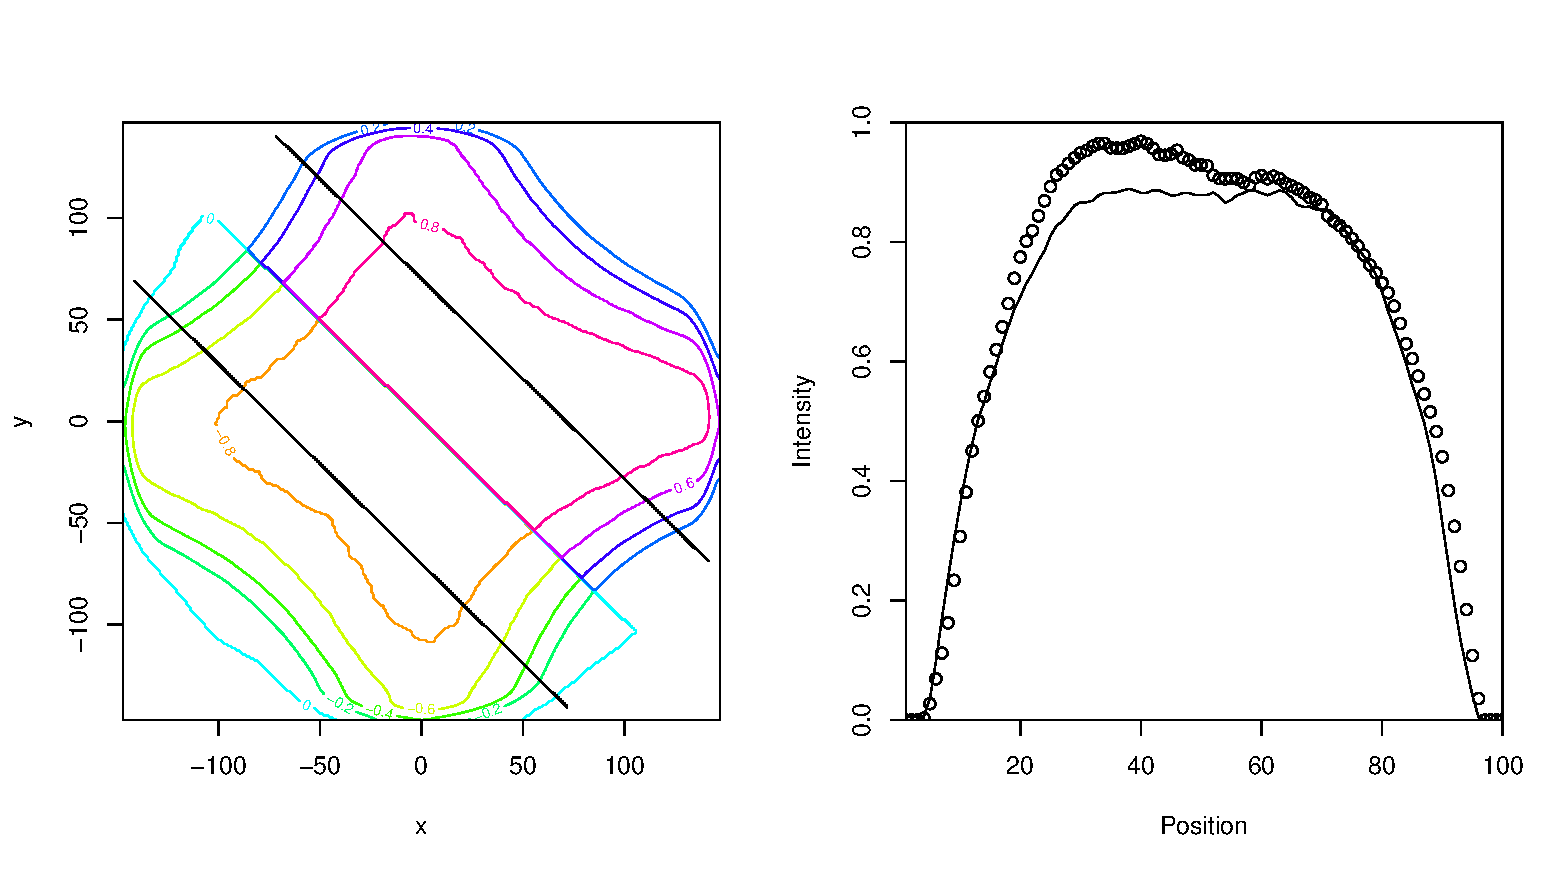
\includegraphics[width=0.38\textwidth]{Figures/90/uniform_rotation/5}}\hspace{0.3in}
\subfigure[]{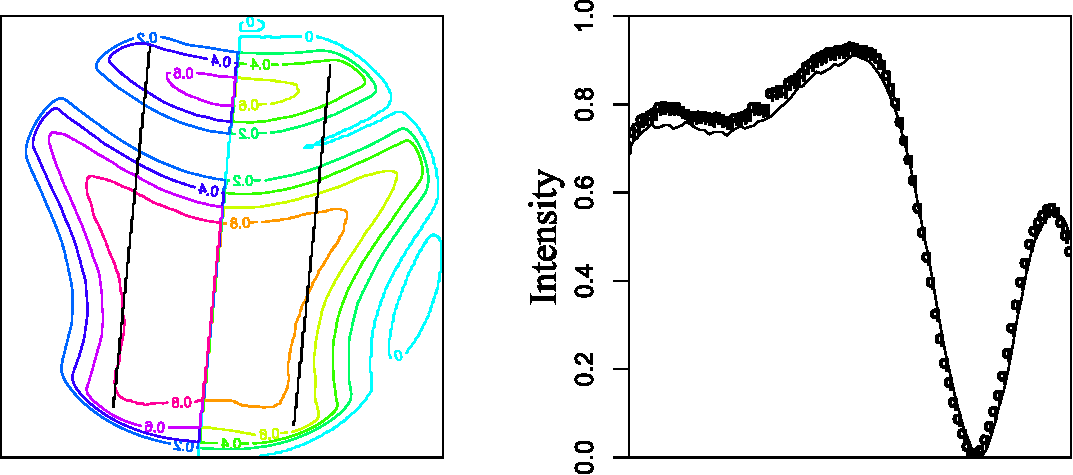
\includegraphics[width=0.38\textwidth]{Figures/90/uniform_rotation/6}}
\end{center}
\caption[Automated tracking of the conoscopic figure rotation]{\label{fig:uniform_rotation}The automated tracking of conoscopic figure rotation. Here, the initial guess (a) and subsequent iterations (b - f) of the azimuthal alignment are shown, along with the pixel intensities of the test lines for the 20 $\mu L/h$ flow conoscopic figure taken from Figure \ref{fig:uniform_data}. After five iterations, the best fit has been achieved, giving an angle of $\phi\approx84^{\circ}$}
\end{figure}

Accordingly, a plot of the conoscopic figure rotation angle as a function of the volumetric flow rate is shown in Figure \ref{fig:uniform_data_plot}, whereby the angles have been calculated for every experimental conoscopic figure in the manner described above. Here, it is far easier to see that the experimental conoscopic figures have rotated through a small minimum, as was predicted by the one dimensional dynamic model. In this figure, the simulated conoscopic figure rotation angle as a function of the simulated volumetric flow rate is also included (red line), along with the average azimuthal distortion as a function of the simulated volumetric flow rate (black dashed line). In order to simulate these curves, a uniform tilt angle of approximately $3^{\circ}$ away from the surface was used, as calculated in Section \ref{sec:calc_tilt}.

\begin{figure}
\begin{center}
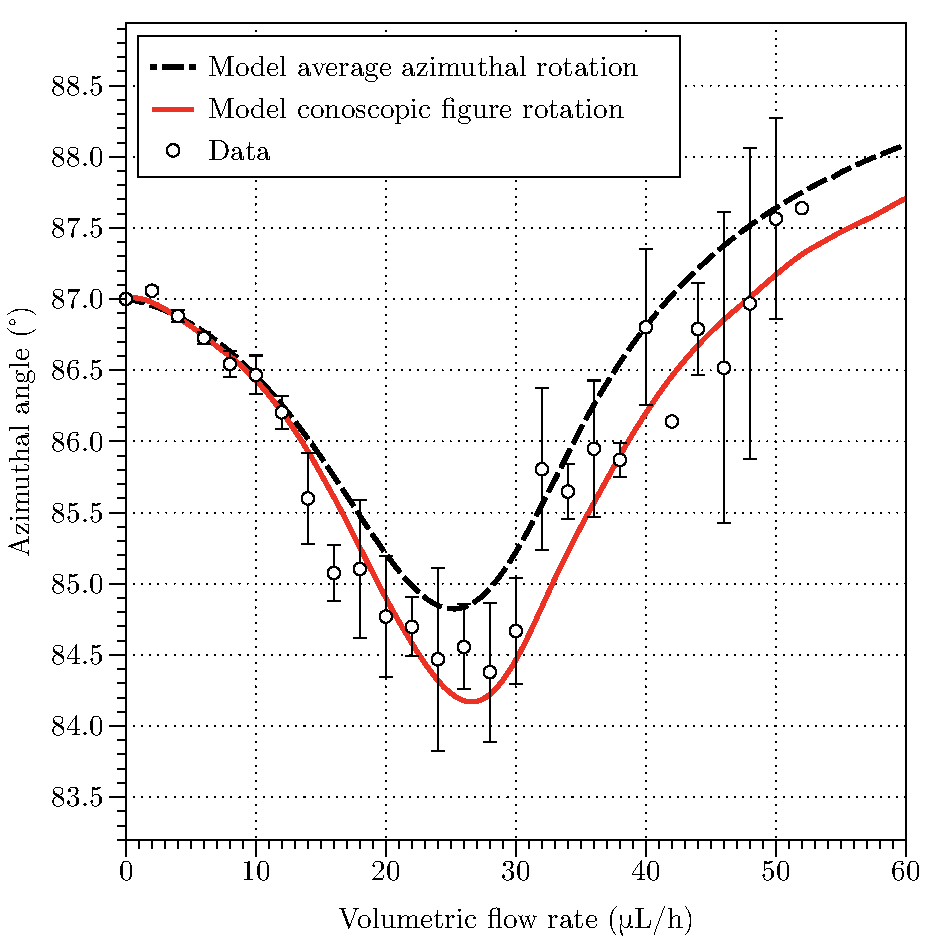
\includegraphics[width=0.65\textwidth]{Figures/90/uniform_data_plot}
\end{center}
\caption[Plot of experimental conoscopic figure rotation as a function of flow rate]{\label{fig:uniform_data_plot}A plot of the conoscopic figure azimuthal angle $\psi$, as a function of volumetric flow rate set at the syringe drive. Simulated conoscopic figure rotation is also depicted by the solid red line (obtained using the same automated routine). The simulated average azimuthal distortion is also shown as a function of the volumetric flow rate (dashed black line).}
\end{figure}

A comparison between the experimental and simulated conoscopic figures is shown in Figure \ref{fig:87_model_data}. Here, the qualitative similarity between the experimental and simulated figures is clear.

\begin{figure}
\begin{center}
\subfigure[0 $\mu$L/h]{\includegraphics[width=0.17\textwidth]{Figures/90/parallel/data/leveled/00}}
\subfigure[0 $\mu$L/h]{\includegraphics[width=0.17\textwidth]{Figures/90/Parallel/87refit/00}}\\
\subfigure[8 $\mu$L/h]{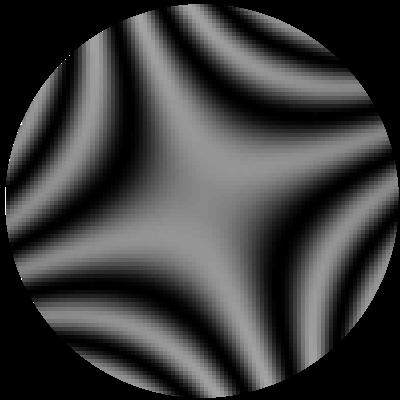
\includegraphics[width=0.17\textwidth]{Figures/90/parallel/data/leveled/04}}
\subfigure[8 $\mu$L/h]{\includegraphics[width=0.17\textwidth]{Figures/90/Parallel/87refit/17}}\\
\subfigure[16 $\mu$L/h]{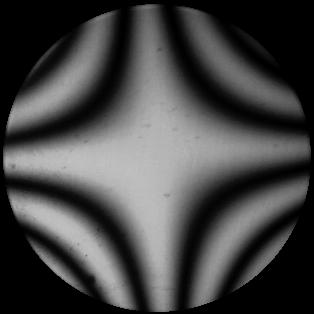
\includegraphics[width=0.17\textwidth]{Figures/90/parallel/data/leveled/08}}
\subfigure[16 $\mu$L/h]{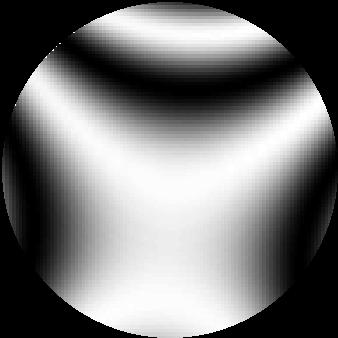
\includegraphics[width=0.17\textwidth]{Figures/90/Parallel/87refit/33}}\\
\subfigure[24 $\mu$L/h]{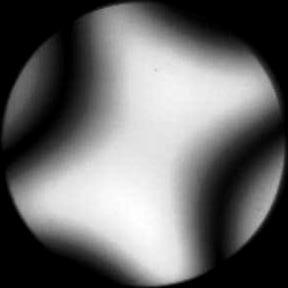
\includegraphics[width=0.17\textwidth]{Figures/90/parallel/data/leveled/12}}
\subfigure[24 $\mu$L/h]{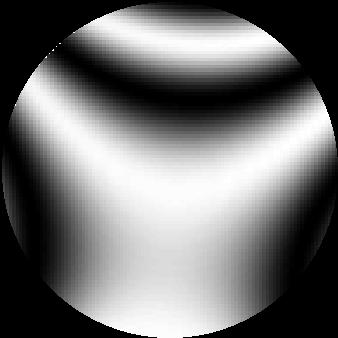
\includegraphics[width=0.17\textwidth]{Figures/90/Parallel/87refit/50}}\\
\subfigure[32 $\mu$L/h]{\includegraphics[width=0.17\textwidth]{Figures/90/parallel/data/leveled/16}}
\subfigure[32 $\mu$L/h]{\includegraphics[width=0.17\textwidth]{Figures/90/Parallel/87refit/67}}\\
\subfigure[40 $\mu$L/h]{\includegraphics[width=0.17\textwidth]{Figures/90/parallel/data/leveled/20}}
\subfigure[40 $\mu$L/h]{\includegraphics[width=0.17\textwidth]{Figures/90/Parallel/87refit/86}}
\end{center}
\caption[Comparison between experimental and simulated conoscopic figures (uniform state)]{\label{fig:87_model_data} A comparison between the experimental and simulated conoscopic figures. Experimental figures are shown in the column on the left and simulated figures are shown in the column on the right. Both are shown for the volumetric flow rate given in the individual figure caption.}
\end{figure}

\subsection{Uniform director profiles}
\label{sec:uniform_state_analysis}
A plot of the simulated $\phi$ and $\theta$ rotations can be seen in Figures \ref{fig:uniform_twist_tilt_profile} (a) and (b). Here, director distortions in both $\phi$ and $\theta$ as a function of position in $z$ and the volumetric flow rate in the cell are shown. For these plots, each line indicates a separate flow rate (or pressure gradient applied across the cell) with the plotted lines ranging from blue to yellow, with blue being zero flow, and yellow being maximum flow.

\begin{figure}
\begin{center}
\subfigure[Twist profile]{\includegraphics[width=0.49\textwidth]{Figures/90/uniform_twist_profile1}}
\subfigure[Tilt profile]{\includegraphics[width=0.49\textwidth]{Figures/90/uniform_tilt_profile1}}
\subfigure[Velocity profile]{\includegraphics[width=0.49\textwidth]{Figures/90/uniform_velocity_profile1}}
\end{center}
\caption[Simulated twist, tilt and velocity profiles (uniform state)]{\label{fig:uniform_twist_tilt_profile} Azimuthal `twist' (a), zenith `tilt' (b) and velocity profiles (c) as a function of position in $z$ and volumetric flow rate (calculated from the simulated pressure gradient). All three figures show curves at regular intervals from blue (no flow) to yellow (maximum flow), going through orange.}
\end{figure}

As has already been discussed with reference to Figure \ref{fig:90_twist_profile_sparce}, the director is seen to distort in Figure \ref{fig:uniform_twist_tilt_profile} (a) in opposite directions in the bottom and top halves of the cell. As was stated earlier, the director can be thought of as azimuthally distorting in one direction (negatively) in more than one half of the cell, while the remainder of the cell distorts azimuthally in the opposite direction (positively). This difference creates the initial small overall azimuthal distortion in the negative direction as shown up to a volumetric flow rate of approximately $28 \mu L/h$ in Figure \ref{fig:uniform_data_plot}. Once the flow rate has reached a critical value, this effect is weakened and ultimately reversed, with more than half of the cell azimuthally distorting in the positive direction, with the overall effect being an increase in the average azimuthal distortion and the creation of the turning point and the rise of the curve back towards $90^{\circ}$ in Figure \ref{fig:uniform_data_plot}.

The physical reason behind this response can be described by the same reasoning suggested by Pieranski and Guyon \cite{Pieranski1974}, as discussed in Chapter \ref{cha:45} for the flow alignment of 5CB initially aligned at $45^{\circ}$ to the flow direction. Here, the director is initially rotated by $3^{\circ}$ away from normal to the flow direction $\left(\phi_0=87^{\circ}\right)$ and anchored at the surface, with a tilt angle of 3 degrees (away from the surface). As such, in the lower half of the cell, the flow induced torque on the director causes it to rotate clockwise towards $\phi=0^{\circ}$, as we expect from the steady state angles and the analysis provided in Chapter \ref{cha:45}. Here, the presence of the $3^{\circ}$ pretilt angle serves to make this azimuthal distortion occur at lower flow rates, as was explained by the simulation of the effect of surface pretilt on azimuthal rotation in Chapter \ref{cha:45} Section \ref{sec:45_vary_tilt}. However, in the top half of the cell, the director is also tilted by $3^{\circ}$, with its top end anchored at the cell boundary (i.e. not in the splayed state simulated in Chapter \ref{cha:45} Section \ref{sec:45_vary_tilt}). In this case, the director can be thought of as being aligned backwards into the flow by $3^{\circ}$. As such, the torque on the director causes it to rotate anti-clockwise in order for it to reach steady state alignment and become parallel to the flow direction at an angle of $\phi=180^{\circ}$ (an allowed steady state alignment angle due to the equivalence of $\mathbf{n}$ and $\mathbf{-n}$) \cite{Horn2003}. This opposite rotation of the director in the lower and upper halves of the cell results in the observation of no net rotation of the conoscopic figure.

In terms of the tilt profile for this geometry, Figure \ref{fig:uniform_twist_tilt_profile} (b) shows the $\theta$ distortion as a function of both flow rate and position in $z$. As is simulated, for the static case (blue line) the cell is aligned at $\theta_0=87^{\circ}$ throughout the cell depth (a value of $3^{\circ}$ tilted away from the surface as estimated from the calculation in Section \ref{sec:calc_tilt}). Again, as the flow rate is increased (towards the yellow line), the director is seen to rotate in the bottom half of the cell to achieve the Leslie angle ($\theta$ begins to saturate at close to $11^{\circ}$ away from planar alignment $\left(\theta_0=90^{\circ}\right)$). In the top half of the cell, the same response is seen, but at a slower rate. For a given flow rate, the director has tilted less towards the Leslie angle in the top half of the cell than in the bottom half of the cell. This again is attributed to the initial alignment and surface anchoring conditions, whereby the director in the top half of the cell must rotate more in an anti-clockwise direction before achieving steady state. At the highest flow rates, the director is seen to come to the Leslie angle in the bottom and top halves of the cell but crucially at the cell mid-plane, the value of $\theta$ is not $90^{\circ}$ but is also tilted some way towards the Leslie angle. This results in the observed translation of the centre of the conoscopic figure away from the centre of the field of view. It is clear that the average tilt angle increases as a function of flow rate, and therefore, the conoscopic figure is seen to translate further as the flow rate is increased.

This chapter will now go on to look at the pressure driven flow response of the director when aligned in the splayed tilt state (Figure \ref{fig:uniform_splayed} (b)) which may be easily fabricated by aligning the glass plate boundaries of the cell so that their rubbing directions are parallel to one another.

\section{Splayed tilt alignment experiment}
\label{sec:splayed}
As a complementary experiment to that described in Section \ref{sec:uniform_experiment}, a cell constructed in the splayed tilted state (Figure \ref{fig:uniform_splayed} (b)) was also fabricated with an initial azimuthal alignment angle of $\phi_0=87^{\circ}$ provided by the mechanical rubbing of the polyimide layer. This geometry creates a splay of the director aligned at an azimuthal angle almost parallel to the $y$ axis, but with a small inclination to the flow direction. This experiment serves to highlight the dramatic difference in the overall director profiles achieved under flow for what is technically a small difference in the initial alignment conditions produced from a rubbed polyimide layer.

As such (and as will be expanded upon in Chapter \ref{cha:diode}) this splayed geometry creates an interesting situation whereby the liquid crystal can be made to flow in two directions upon which it experiences different initial alignment conditions relative to the flow direction. These two directions can be described `with' the splay that is created (flow in the positive $x$ direction) and `against' the created splay (flow in the negative $x$ direction). As will be seen later in this section, the results of these experiments closely resemble those presented in Chapter \ref{cha:45}, where the director was initially aligned at $\phi_0=45^{\circ}$. As a result of this, the conoscopic figures presented here differ from those presented earlier in this chapter (Section \ref{sec:uniform_experiment}) for the uniformly tilted alignment condition. In essence, this experiment shows no translation of the centre of the figure away from the field of view, whilst as previously discovered, the conoscopic figure rotates about its centre. The corresponding simulations are also made, using the same computational model described in previous chapters. This gives some insight in to the possible director profiles created under flow.

As before, the experimental conditions used here are identical to those described earlier in this chapter, and also for the flow experiment ($\phi_0=45^{\circ}$) described in Chapter \ref{cha:45}. The results of which are described in the next two sub sections, titled separately `With' and `Against' the splay.

\subsection{`With' the splay}
Figure \ref{fig:splay_with_data} shows the experimental conoscopic figures as a function of the volumetric flow rate set at the syringe pump (with the flow rate shown in the individual figure caption).

As seen before, here the conoscopic figure is seen to rotate into the flow direction as the flow rate is increased. Starting with an initial alignment of close to $\psi=87^{\circ}$ (Figure \ref{fig:splay_with_data} (a)) and rotating around to approximately $\psi=37^{\circ}$ (Figure \ref{fig:splay_with_data} (k)). Similarly, there is no observed translation of the centre of the conoscopic figure from the field of view, suggesting that the \textit{average} tilt angle within the cell has also been maintained at $\theta=90^{\circ}$ (planar). 

\begin{figure}
\begin{center}
\subfigure[0 $\mu$L/h]{\includegraphics[width=0.17\textwidth]{Figures/90/Splay/with/cropped/00a}}
%\subfigure[2 $\mu$L/h]{\includegraphics[width=0.17\textwidth]{Figures/90/Splay/with/cropped/01}}
\subfigure[4 $\mu$L/h]{\includegraphics[width=0.17\textwidth]{Figures/90/Splay/with/cropped/02}}
%\subfigure[6 $\mu$L/h]{\includegraphics[width=0.17\textwidth]{Figures/90/Splay/with/cropped/03}}
\subfigure[8 $\mu$L/h]{\includegraphics[width=0.17\textwidth]{Figures/90/Splay/with/cropped/04}}
%\subfigure[10 $\mu$L/h]{\includegraphics[width=0.17\textwidth]{Figures/90/Splay/with/cropped/05}}
\subfigure[12 $\mu$L/h]{\includegraphics[width=0.17\textwidth]{Figures/90/Splay/with/cropped/06}}
%\subfigure[14 $\mu$L/h]{\includegraphics[width=0.17\textwidth]{Figures/90/Splay/with/cropped/07}}
\subfigure[16 $\mu$L/h]{\includegraphics[width=0.17\textwidth]{Figures/90/Splay/with/cropped/08}}
%\subfigure[18 $\mu$L/h]{\includegraphics[width=0.17\textwidth]{Figures/90/Splay/with/cropped/09}}
\subfigure[20 $\mu$L/h]{\includegraphics[width=0.17\textwidth]{Figures/90/Splay/with/cropped/10a}}
%\subfigure[22 $\mu$L/h]{\includegraphics[width=0.17\textwidth]{Figures/90/Splay/with/cropped/11}}
\subfigure[24 $\mu$L/h]{\includegraphics[width=0.17\textwidth]{Figures/90/Splay/with/cropped/12}}
%\subfigure[26 $\mu$L/h]{\includegraphics[width=0.17\textwidth]{Figures/90/Splay/with/cropped/13}}
\subfigure[28 $\mu$L/h]{\includegraphics[width=0.17\textwidth]{Figures/90/Splay/with/cropped/14}}
%\subfigure[30 $\mu$L/h]{\includegraphics[width=0.17\textwidth]{Figures/90/Splay/with/cropped/15}}
\subfigure[32 $\mu$L/h]{\includegraphics[width=0.17\textwidth]{Figures/90/Splay/with/cropped/16}}
%\subfigure[34 $\mu$L/h]{\includegraphics[width=0.17\textwidth]{Figures/90/Splay/with/cropped/17}}
\subfigure[36 $\mu$L/h]{\includegraphics[width=0.17\textwidth]{Figures/90/Splay/with/cropped/18}}
%\subfigure[38 $\mu$L/h]{\includegraphics[width=0.17\textwidth]{Figures/90/Splay/with/cropped/19}}
\subfigure[40 $\mu$L/h]{\includegraphics[width=0.17\textwidth]{Figures/90/Splay/with/cropped/20a}}
%\subfigure[42 $\mu$L/h]{\includegraphics[width=0.17\textwidth]{Figures/90/Splay/with/cropped/21}}
\end{center}
\caption[Experimental conoscopic figures for flow `with' the splay]{\label{fig:splay_with_data}Flow `with' the splay. Experimental conoscopic interference figures for the cell rubbed at $\phi_0=87^{\circ}$ in parallel directions in order to create a splayed director geometry. Here, an overall rotation of the conoscopic figure is seen as a function of the volumetric flow rate set by the syringe drive (shown in the individual figure caption).}
\end{figure}

Simulated director profiles are shown in Figure \ref{fig:splayed_with_twist_tilt_profile}. Here, the simulation confirms, as expected, that the director has azimuthally distorted to align parallel to the flow direction in the bulk of the sample. This is seen in Figure \ref{fig:splayed_with_twist_tilt_profile} (a) by the curves in the central portion of the cell moving towards an azimuthal angle of $\phi=0^{\circ}$ as the flow rate is increased. Here, it is also hinted at that the small degree of pretilt is causing the director to rotate towards $\phi=0^{\circ}$ at lower flow rates than would be experienced if the director were aligned with no pretilt angle (heading towards the Pieranski-Guyon instability described in Chapter \ref{cha:45} where the effect of pretilt is demonstrated in Figure \ref{fig:45_vary_tilt}). This is shown in Figure \ref{fig:splayed_with_twist_tilt_profile} (a) by the initially small change in $\phi$ as a function of cell depth (the second blue line), followed by a much larger change (the third blue line) before saturating at an angle almost parallel to the flow direction (yellow line). The results of this sudden rotation are also seen in the average of the azimuthal rotation by the conoscopic figures at lower flow rates (shown in Figures \ref{fig:splay_with_data} (a) - (e)).

As seen before, the director is also simulated to have rotated to achieve the Leslie angle of opposite signs in the top and bottom halves of the cell. This is shown by the distortion of the curves depicted in Figure \ref{fig:splayed_with_twist_tilt_profile} (b). Much like those shown for the $\phi_0=45^{\circ}$ described in Chapter \ref{cha:45}, the tilt angle of the director saturates (at the highest flow rates) at angles approximately $11^{\circ}$ away from the planar position ($\theta=90^{\circ}$) in the top and bottom halves of the cell.

Figure \ref{fig:splayed_with_twist_tilt_profile} (c) also depicts simulated velocity profiles as a function of the cell depth and pressure gradient. Again, the typical parabolic flow profile is recovered, whereby non-slip boundary conditions dictate that the velocity must go to zero at the cell walls.

A plot of the average rotation angle of the conoscopic figures as a function of the volumetric flow rate (for both data and simulated figures) can be seen later on in Figure \ref{fig:uniform_data_plot}.

\begin{figure}
\begin{center}
\subfigure[Twist profile]{\includegraphics[width=0.49\textwidth]{Figures/90/splay/with/twist_profile}}
\subfigure[Tilt profile]{\includegraphics[width=0.49\textwidth]{Figures/90/splay/with/tilt_profile}}
\subfigure[Velocity profile]{\includegraphics[width=0.49\textwidth]{Figures/90/splay/with/velocity_profile}}
\end{center}
\caption[Simulated twist, tilt and velocity profiles for flow `with' the splay]{\label{fig:splayed_with_twist_tilt_profile}Simulated azimuthal `twist' (a), zenithal `tilt' (b) and velocity profiles (c) as a function of position in $z$ and volumetric flow rate (calculated from the simulated pressure gradient) for flow `with' the splay. All three figures show curves at regular intervals in the prescribed pressure gradient, from blue (no flow) to yellow (maximum flow), going through orange.}
\end{figure}

\subsection{`Against' the splay}
Figure \ref{fig:splay_against_data} depicts the experimental conoscopic figures as a function of the volumetric flow rate set at the syringe pump (shown in the individual figure captions) for flow against the splay (in the negative $x$ direction, from right to left as indicated by the arrows)\footnote{The difference in the 0 $\mu L/h$ capture between Figure \ref{fig:splay_with_data} (a) and Figure \ref{fig:splay_against_data} (a) is due to the experimental difficulty in rotating the cell so that flow could be applied in the opposite direction. In doing so, the area of the cell being sampled has changed, with variations in cell thickness causing the dark fringes to move.}. Here, the figures are seen to have an initial azimuthal alignment of close to $\psi=87^{\circ}$ (Figure \ref{fig:splay_against_data} (a)) and rotate around, through $\psi=90^{\circ}$, to approximately $\psi=130^{\circ}$ (Figure \ref{fig:splay_against_data} (k)). Similarly, as for flow `with' the splay, Figures \ref{fig:splay_against_data} (a) to (k) show that there is no observed translation of the centre of the conoscopic figure from the field of view, suggesting that the \textit{average} tilt angle within the cell has also been maintained at $\theta=90^{\circ}$ (planar).

\begin{figure}
\begin{center}
\subfigure[0 $\mu$L/h]{\includegraphics[width=0.17\textwidth]{Figures/90/Splay/against/cropped/levelled/00a}}
%\subfigure[2 $\mu$L/h]{\includegraphics[width=0.17\textwidth]{Figures/90/Splay/with/cropped/01}}
\subfigure[4 $\mu$L/h]{\includegraphics[width=0.17\textwidth]{Figures/90/Splay/against/cropped/levelled/02}}
%\subfigure[6 $\mu$L/h]{\includegraphics[width=0.17\textwidth]{Figures/90/Splay/with/cropped/03}}
\subfigure[8 $\mu$L/h]{\includegraphics[width=0.17\textwidth]{Figures/90/Splay/against/cropped/levelled/04}}
%\subfigure[10 $\mu$L/h]{\includegraphics[width=0.17\textwidth]{Figures/90/Splay/with/cropped/05}}
\subfigure[12 $\mu$L/h]{\includegraphics[width=0.17\textwidth]{Figures/90/Splay/against/cropped/levelled/06}}
%\subfigure[14 $\mu$L/h]{\includegraphics[width=0.17\textwidth]{Figures/90/Splay/with/cropped/07}}
\subfigure[16 $\mu$L/h]{\includegraphics[width=0.17\textwidth]{Figures/90/Splay/against/cropped/levelled/08a}}
%\subfigure[18 $\mu$L/h]{\includegraphics[width=0.17\textwidth]{Figures/90/Splay/with/cropped/09}}
\subfigure[20 $\mu$L/h]{\includegraphics[width=0.17\textwidth]{Figures/90/Splay/against/cropped/levelled/10}}
%\subfigure[22 $\mu$L/h]{\includegraphics[width=0.17\textwidth]{Figures/90/Splay/with/cropped/11}}
\subfigure[24 $\mu$L/h]{\includegraphics[width=0.17\textwidth]{Figures/90/Splay/against/cropped/levelled/12}}
%\subfigure[26 $\mu$L/h]{\includegraphics[width=0.17\textwidth]{Figures/90/Splay/with/cropped/13}}
\subfigure[28 $\mu$L/h]{\includegraphics[width=0.17\textwidth]{Figures/90/Splay/against/cropped/levelled/14}}
%\subfigure[30 $\mu$L/h]{\includegraphics[width=0.17\textwidth]{Figures/90/Splay/with/cropped/15}}
\subfigure[32 $\mu$L/h]{\includegraphics[width=0.17\textwidth]{Figures/90/Splay/against/cropped/levelled/16}}
%\subfigure[34 $\mu$L/h]{\includegraphics[width=0.17\textwidth]{Figures/90/Splay/with/cropped/17}}
\subfigure[36 $\mu$L/h]{\includegraphics[width=0.17\textwidth]{Figures/90/Splay/against/cropped/levelled/18}}
%\subfigure[38 $\mu$L/h]{\includegraphics[width=0.17\textwidth]{Figures/90/Splay/with/cropped/19}}
\subfigure[40 $\mu$L/h]{\includegraphics[width=0.17\textwidth]{Figures/90/Splay/against/cropped/levelled/20a}}
%\subfigure[42 $\mu$L/h]{\includegraphics[width=0.17\textwidth]{Figures/90/Splay/with/cropped/21}}
\end{center}
\caption[Experimental conoscopic figures for flow `against' the splay]{\label{fig:splay_against_data}Flow `against' the splay. Experimental conoscopic interference figures for the cell rubbed at $\phi_0=87^{\circ}$ in parallel directions in order to create a splayed director geometry. Here, an overall rotation of the conoscopic figure is seen as a function of the volumetric flow rate set by the syringe drive (shown in the individual figure caption).}
\end{figure}

Again, Figure \ref{fig:splayed_against_twist_tilt_profile} shows the appropriately simulated director profiles. Much like for the case of flow `with' the splay, Figure \ref{fig:splayed_against_twist_tilt_profile} (a) depicts the simulated twist profile as a function of the cell depth. It is seen that the director rotates backwards through $90^{\circ}$ towards an angle of $\phi=180^{\circ}$. Here, more pronounced, is the jump in azimuthal rotation between the first two simulated pressure gradients (first two blue lines) resulting in a `kick' of the azimuthal rotation of the director. This is clearly also seen in the captured conoscopic figures where at low flow rates (Figure \ref{fig:splay_against_data} (a) to (e)) the conoscopic figure has barely rotated, until a sudden kick in the rotation at approximately 20 $\mu L/h$ (Figure \ref{fig:splay_against_data} (f)).

\begin{figure}
\begin{center}
\subfigure[Twist profile]{\includegraphics[width=0.49\textwidth]{Figures/90/splay/against/twist_profile}}
\subfigure[Tilt profile]{\includegraphics[width=0.49\textwidth]{Figures/90/splay/against/tilt_profile}}
\subfigure[Velocity profile]{\includegraphics[width=0.49\textwidth]{Figures/90/splay/against/velocity_profile}}
\end{center}
\caption[Simulated twist, tilt and velocity profiles for flow `against' the splay]{\label{fig:splayed_against_twist_tilt_profile}Simulated azimuthal `twist' (a), zenith `tilt' (b) and velocity profiles (c) as a function of position in $z$ and volumetric flow rate (calculated from the simulated pressure gradient) for flow `against' the splay. All three figures show curves at regular intervals in the prescribed pressure gradient, from blue (no flow) to yellow (maximum flow), going through orange.}
\end{figure}

Figure \ref{fig:splayed_against_twist_tilt_profile} (b) also depicts the simulated director tilt profile. Again, it is seen that the director appears to achieve the Leslie angle of opposite signs in the top and bottom halves of the cell (resulting in no translation of the centre of the figure from the field of view). This is shown by the distortion of the curves depicted in Figure \ref{fig:splayed_against_twist_tilt_profile} (b). Again, much like those shown for the $\phi_0=45^{\circ}$ case described in Chapter \ref{cha:45}, the tilt angle of the director saturates (at the highest flow rates) at angles approximately $11^{\circ}$ away from the planar position ($\theta=90^{\circ}$) in the top and bottom halves of the cell. Here however, the less sensitive rotation at lower flow rates (described above) is also seen in the tilt profile. As discussed in Chapter \ref{cha:45}, it is not until the director rotates away from planar alignment that there is significant torque on the molecules to begin the azimuthal rotation.

Figure \ref{fig:splayed_against_twist_tilt_profile} (c) also depicts the simulated velocity profiles, here negative, as the pressure gradient has been prescribed to produce flow in the opposite direction to that shown for flow `with' the splay.

Figure \ref{fig:with_against_data_plot} is a plot of the rotation angle of the conoscopic figures depicted in Figures \ref{fig:splay_with_data} and \ref{fig:splay_against_data} calculated from the automated tracking routine as previously described in (Chapter \ref{cha:45}) and Section \ref{sec:uniform_con_rot} of this chapter. Included are simulated conoscopic figure rotations calculated from the same one dimensional model as used in Chapter \ref{cha:45}.

The response of the average azimuthal rotation for flow `with' and `against' the splay is clear to see. As expected, it is quantitatively clear that for flow in both directions, there is limited rotation at low flow rates, before the rate of change of rotation angle with flow rate increases at higher flow rates. This is particularly clear in the flow `against' curve where at low flow rates the figure barely rotates up to a flow rate of approximately 20 $\mu L/h$ before rapidly distorting, as is qualitatively clear from the data captures shown in Figure \ref{fig:splay_against_data}.

\begin{figure}
\begin{center}
\includegraphics[width=0.65\textwidth]{Figures/90/with_against_data_plot.pdf}
\end{center}
\caption[A plot of experimental conoscopic figure rotation as a function of flow rate for flow `with' and `against' the splay]{\label{fig:with_against_data_plot}A plot of the conoscopic figure azimuthal angle $\psi$, as a function of the volumetric flow rate set at the syringe drive for flow `with' and `against' the splay. Simulated conoscopic figure rotation is also depicted by the solid lines (obtained using the same automated routine).}
\end{figure}

\section{Conclusions}
In this chapter it has been demonstrated that for the pressure driven flow of the nematic liquid crystal 5CB, the presence of a small degree of surface pretilt, which may lead to different symmetries of the static director profile, can greatly affect the director profile in the bulk of the sample when the initial azimuthal alignment is not normal to the flow direction.

The same small degree of pretilt in the uniformly aligned state (Section \ref{sec:uniform_experiment}) appears to produce entirely opposite azimuthal distortions of the director about the cell mid-plane. At low flow rates there is a small net rotation in one direction and at high flow rates in the other. For the splayed state (Section \ref{sec:splayed}), no net tilting of the director is observed, yet a positive net azimuthal distortion is seen. In contrast, for the uniform state, a net tilt distortion of the director is observed, but no net azimuthal distortion is seen. This difference in director distortion results in completely distinct optical conoscopic figures, whereby one (splayed state) shows a rotation and the other (uniform state) shows a lateral translation and small rotation minimum.

It can be argued that, much like the findings of Horn \textit{et al.} \cite{Horn2003}, these results highlight the extreme sensitivity of the flowing director orientation to only a few degrees of surface pretilt and importantly when using an aligning layer such as a rubbed polyimide, one should take care in making the common assumption that the director is truly planar.
